% Created 2023-03-10 ven. 14:10
% Intended LaTeX compiler: pdflatex
\documentclass[presentation]{beamer}
\usepackage[utf8]{inputenc}
\usepackage[T1]{fontenc}
\usepackage[french]{babel}
\usepackage[labelformat=empty]{caption}
\usepackage{verbatim}
\definecolor{purple_wada}{RGB}{128,71,189} %   #8047bdff
\definecolor{links}{HTML}{2A1B81}
\useoutertheme{infolines}
%
% Beamer options
%
\setbeamertemplate{caption}{\raggedright\insertcaption\par}
\setbeamercovered{transparent}
\setbeamertemplate{section in toc}[sections numbered]
\setbeamertemplate{subsection in toc}[square]
\setbeamertemplate{navigation symbols}{}
\setbeamercolor{section in head/foot}{bg=purple_wada, fg=white}
\setbeamercolor{subsection in head/foot}{bg=white, fg=purple_wada}
\setbeamercolor{title in head/foot}{fg=purple_wada,bg=white}
\setbeamercolor{author in head/foot}{fg=white,bg=purple_wada}
\setbeamercolor{date in head/foot}{fg=white,bg=purple_wada}
\setbeamercolor{frametitle}{fg=purple_wada,bg=white}
\setbeamercolor{block title}{fg=purple_wada,bg=white}
%
% Adding frame at each section
%
\AtBeginSubsection[]
{
\begin{frame}
\frametitle{Sommaire}
\tableofcontents[currentsection,currentsubsection]
\end{frame}
}
\usetheme{default}
\author{Doc. Malik Koné}
\date{\today}
\title{Blockchains et Cryptographie}
\hypersetup{
 pdfauthor={Doc. Malik Koné},
 pdftitle={Blockchains et Cryptographie},
 pdfkeywords={},
 pdfsubject={},
 pdfcreator={Emacs 28.2 (Org mode 9.5.5)}, 
 pdflang={French}}
\begin{document}

{
  \usebackgroundtemplate{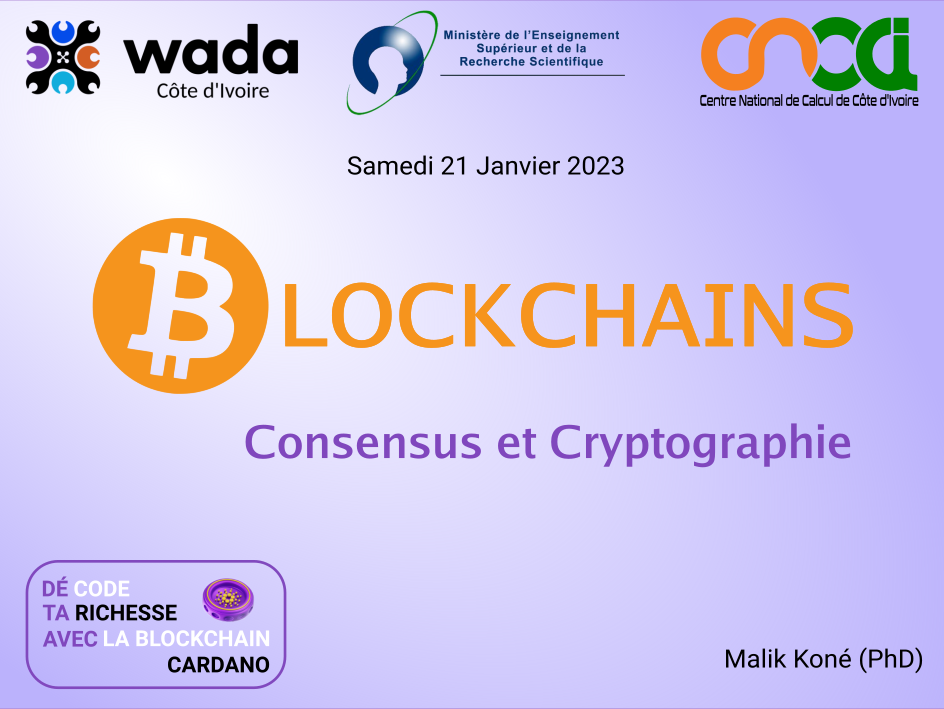
\includegraphics[height=\paperheight]{./page_de_garde_wadaci_j2a}}
  \frame[plain]{
  }
}

\section{Introduction}
\label{sec:orgec0d3ac}
\subsection{De quoi allons-nous parler ?}
\label{sec:orge94a8da}
\begin{frame}[label={sec:orgbe157e8}]{De quoi allons-nous parler ?}
\begin{center}
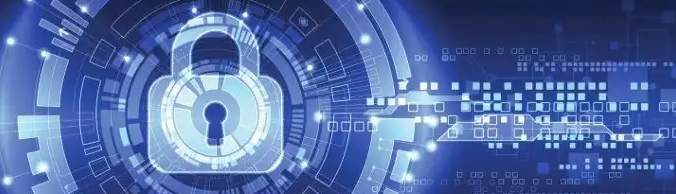
\includegraphics[width=\textwidth]{Images/consensus_cryptographie.png}
\end{center}
\begin{columns}
\begin{column}{0.46\columnwidth}
\begin{block}<1->{Cryptographie \& Consensus}
\begin{itemize}
\item <1>Outils de la cryptographie
\item <1>Systèmes distribués
\item <1>Les différents Consensus
\end{itemize}
\end{block}
\end{column}

\begin{column}{0.54\columnwidth}
\begin{block}<1->{Universalité et Smart-contracts}
\begin{itemize}
\item <0> Applications distribuées (dApp)
\item <0> Etherum et Cardano
\item <0> Quelles applications ?
\end{itemize}
\end{block}
\end{column}
\end{columns}
\end{frame}
\subsection{C'est quoi déjà la blockchain Bitcoin}
\label{sec:org37da688}
\begin{frame}[label={sec:org26c2e95}]{Une chaine de blocs}
\begin{block}<1->{}
\begin{figure}[ht]
   \centering
   \includegraphics<1>[width=\textwidth]{Images/anatomy-of-a-chain-1.png}
   \includegraphics<2>[width=.3\textwidth]{Images/anatomy-of-a-chain-1.png}   
\end{figure}
\end{block}

\begin{block}<2>{Maintenu par ses utilisateurs}
     \only<2>{     
Empereurs,  Élus,  Mineurs, vous et moi.
}

\begin{block}<2>{}
\only<2>{
\begin{figure}[ht]
  \centering
  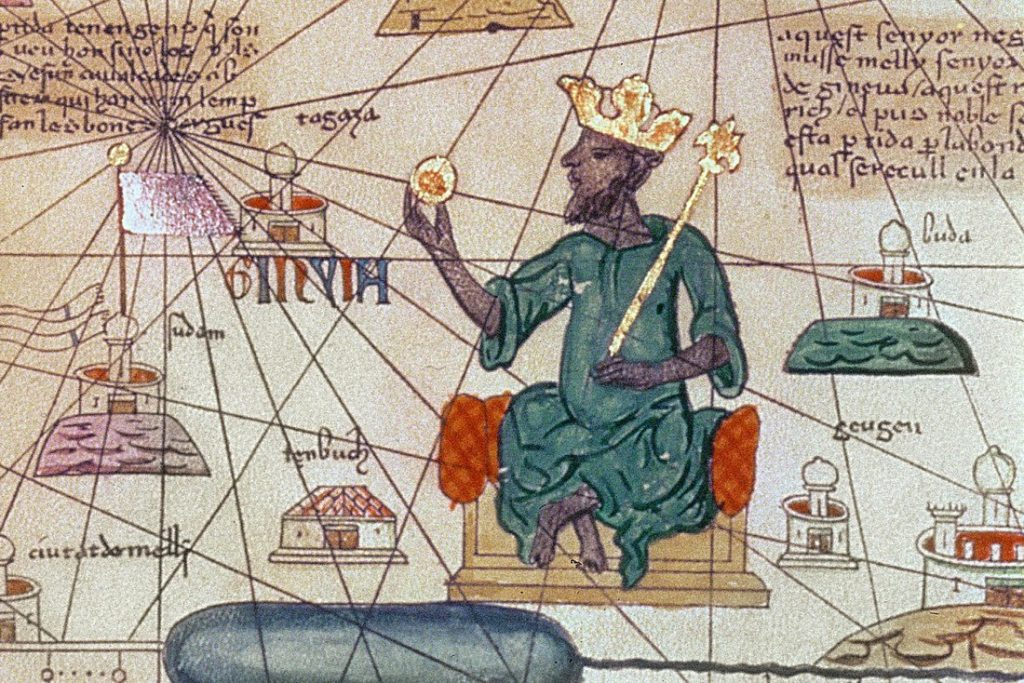
\includegraphics[width=.25\textwidth]{Images/user_empereur}
  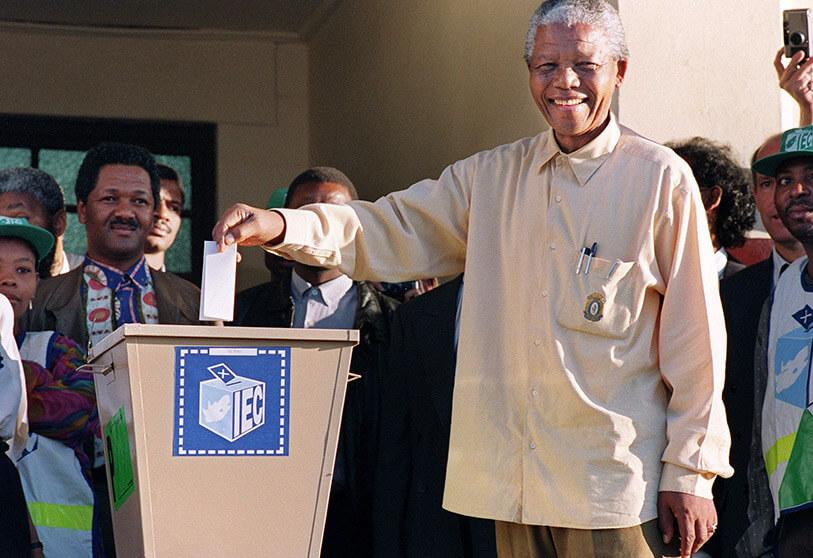
\includegraphics[width=.25\textwidth]{Images/user_elu}
  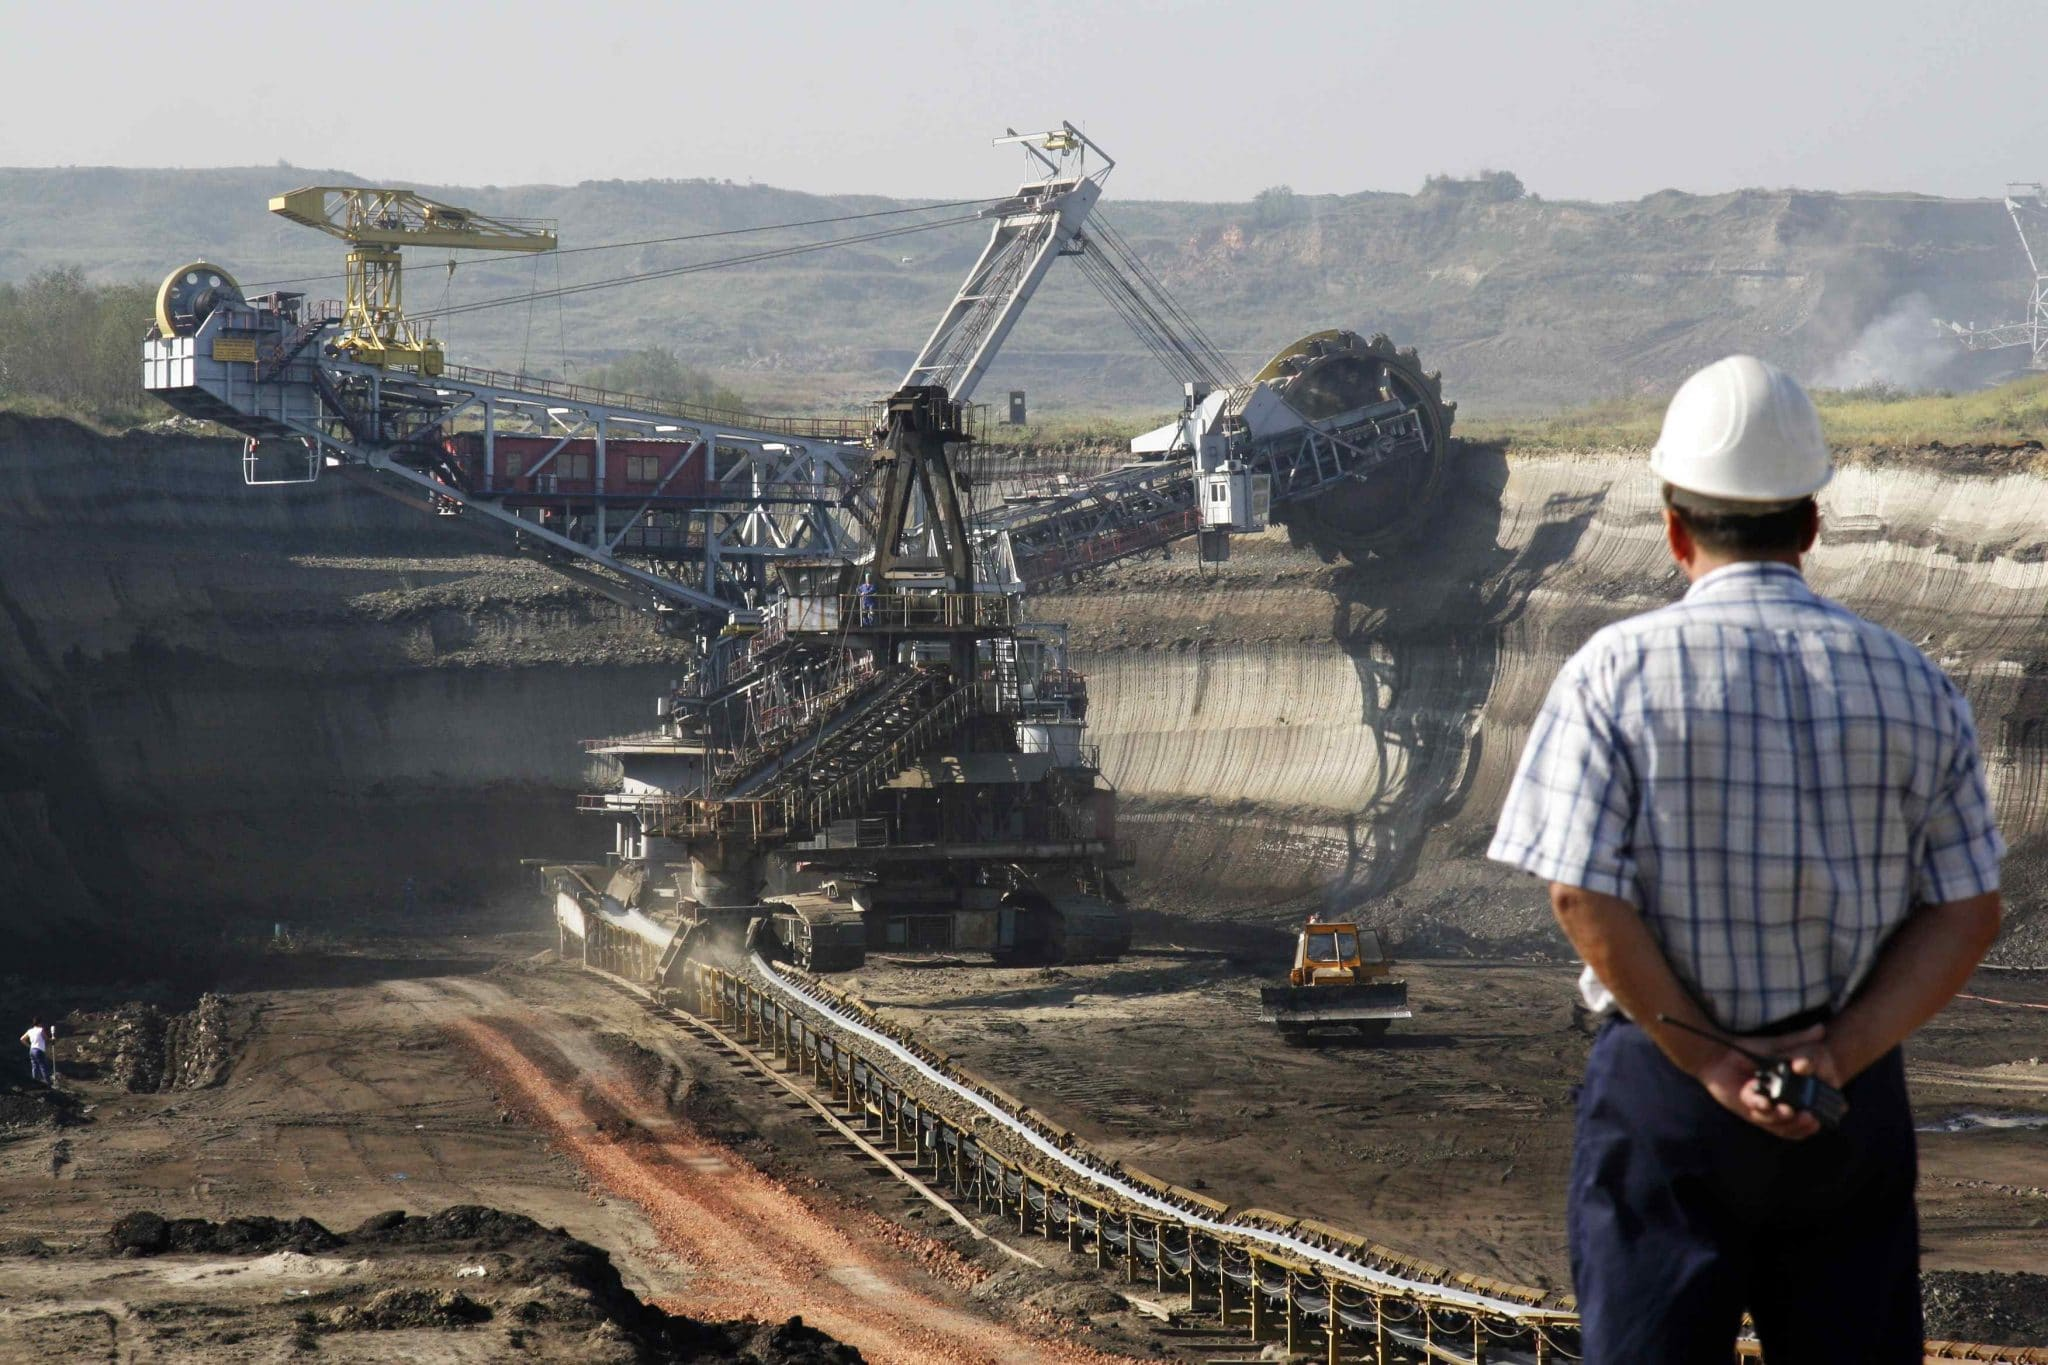
\includegraphics[width=.25\textwidth]{Images/user_mineur2}    
  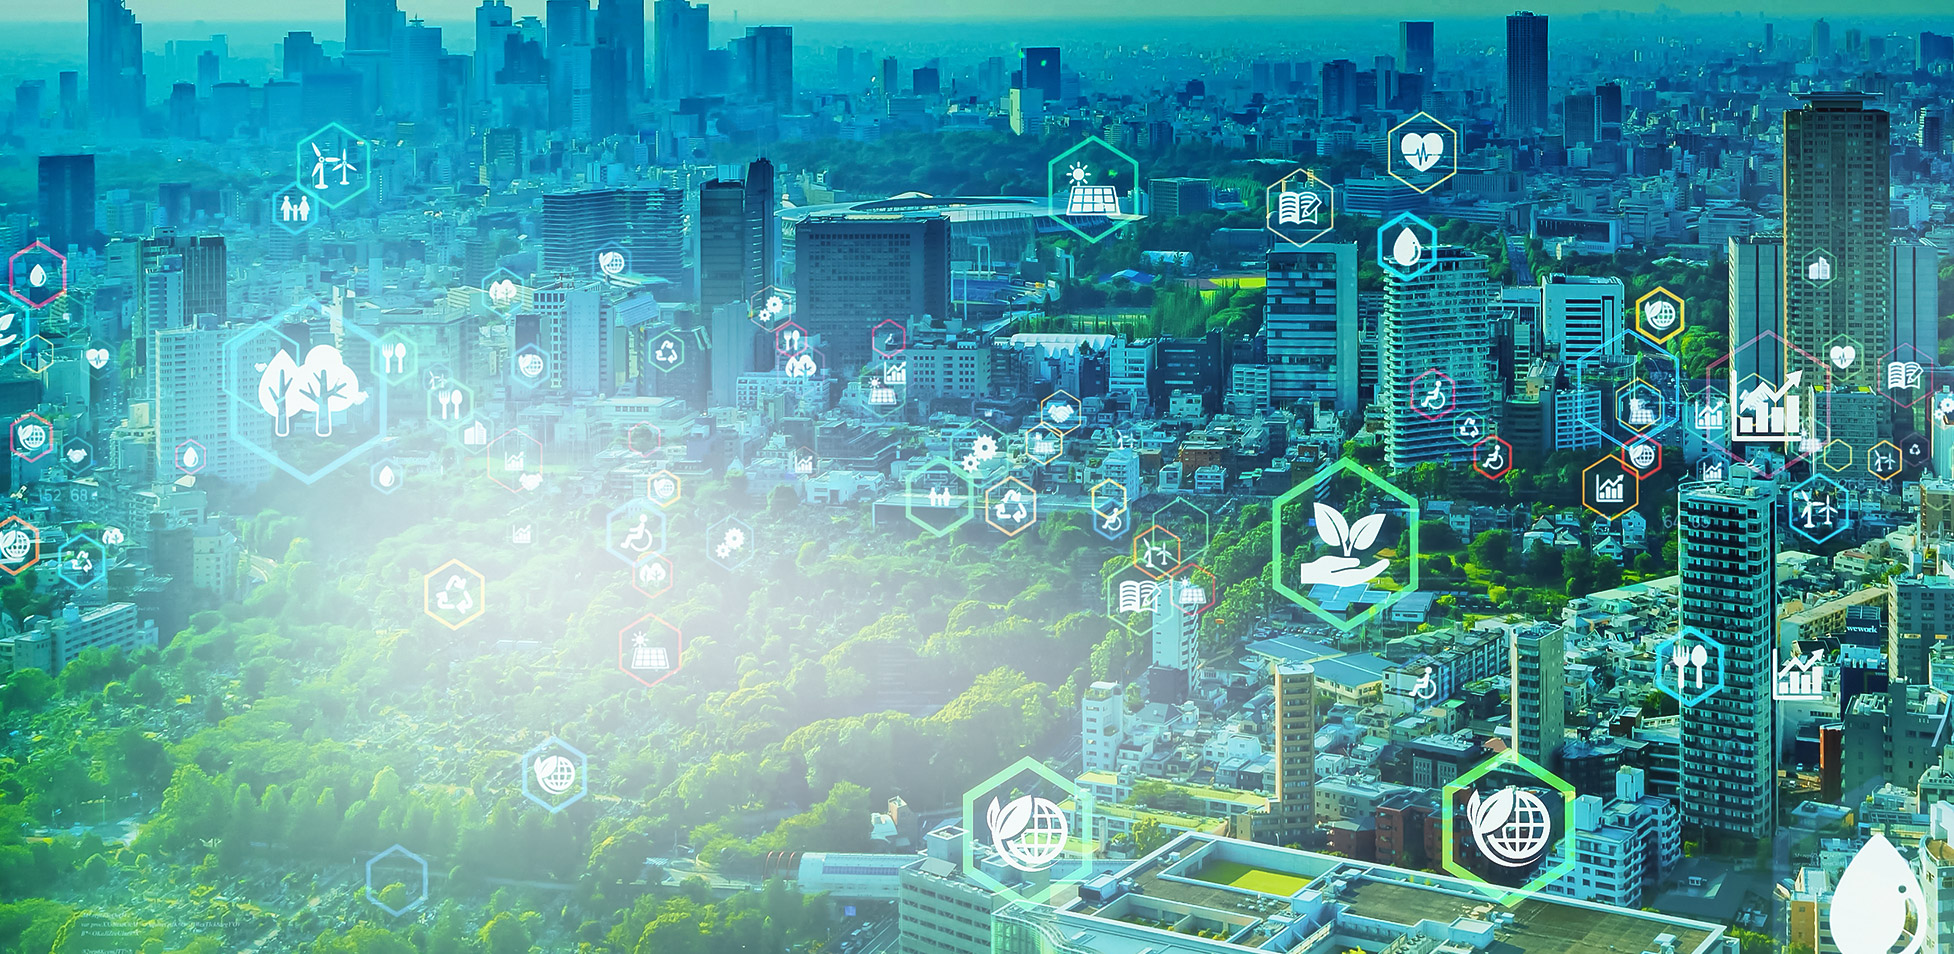
\includegraphics[width=.24\textwidth]{Images/user_user2}
\end{figure}
}
\end{block}
\end{block}
\end{frame}

\begin{frame}[label={sec:org085dd1b}]{C'est un DLT : \emph{Distributed Ledger Technology}}
\begin{figure}[ht]
   \centering
\includegraphics<1>[width=.6\textwidth]{Images/tx}
   \includegraphics<2>[width=.6\textwidth]{Images/block}
   \includegraphics<3>[width=\textwidth]{Images/Anatomy-of-a-block2}    
   \includegraphics<4>[width=\textwidth]{Images/anatomy-of-a-chain-1}
 \end{figure}

\only<1>{
\href{https://andersbrownworth.com/blockchain/tokens}{Tx}:  ".00012300 BTC pour Binta, signé Amadou"
}
\only<2>{
Les mineurs inclu la \href{https://andersbrownworth.com/blockchain/tokens}{tx dans un bloc} et cherchent un \alert{bon} \emph{nonce}
}
\only<3>{
Le 1\ier{} mineur à gagner un \alert{bon} \emph{nonce}, annonce son bloc
\begin{itemize}
\item avec une récompense (\href{https://andersbrownworth.com/blockchain/coinbase}{coinbase})
\item c'est un \alert{élu} (ou leader)
\end{itemize}
}
\only<4>{
Les autres mineurs:
\begin{itemize}
\item Vérifient le bloc
\item Ajoutent le nouveau block \alert{a la plus longue chaine}
\item Puis une nouvelle \alert{loterie} commence.
\end{itemize}

}      
\end{frame}

\section{La cryptographie au service de la blockchain}
\label{sec:orga8cb93b}
\subsection{Transactions (tx)}
\label{sec:org3c51484}
\begin{frame}[label={sec:org1c6804f}]{Validité d'une transaction}
\begin{block}{Qu'est qui rend une transaction valide ?}
\end{block}
\end{frame}
\begin{frame}[label={sec:orge385b69}]{Validité d'une transaction}
\begin{block}{Qu'est qui rend une transaction valide ?}
\end{block}
\begin{columns}
\begin{column}{0.4\columnwidth}
\begin{block}<1->{Il faut \ldots{}}
\begin{itemize}
\item Des fonds disponibles
\item Une identié  (signature)
\item Pas de duplication
\item <2> un compte bancaire ?
\end{itemize}
\end{block}
\end{column}
\begin{column}{0.6\columnwidth}
\begin{block}<2->{Confiance !}
\only<2>{
\begin{figure}[htbp]
\centering
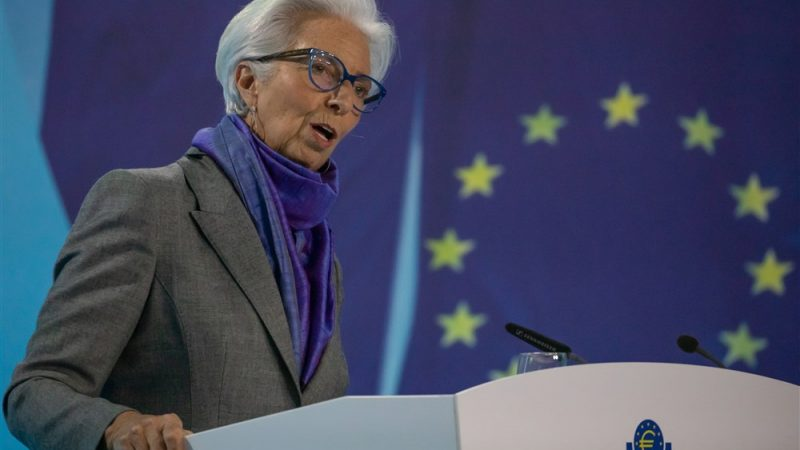
\includegraphics[width=.9\textwidth]{Images/bce_lagarde.jpg}
\caption{en Mme. La-Garde ?}
\end{figure}
}
\end{block}
\end{column}
\end{columns}
\end{frame}


\begin{frame}[label={sec:orgb29dfe4}]{Le Modèle des UTXO : Unspent Transaction Output}
\begin{block}{Les UTXO sont comme des tirelires}
\only<1>{
\begin{figure}[htbp]
\centering

\includegraphics[height=.6\textheight]{Images/tirelire.png}
\caption{Connaître le contenu de sa tirelire}
\end{figure}
}
\only<2>{
\begin{figure}[htbp]
\centering
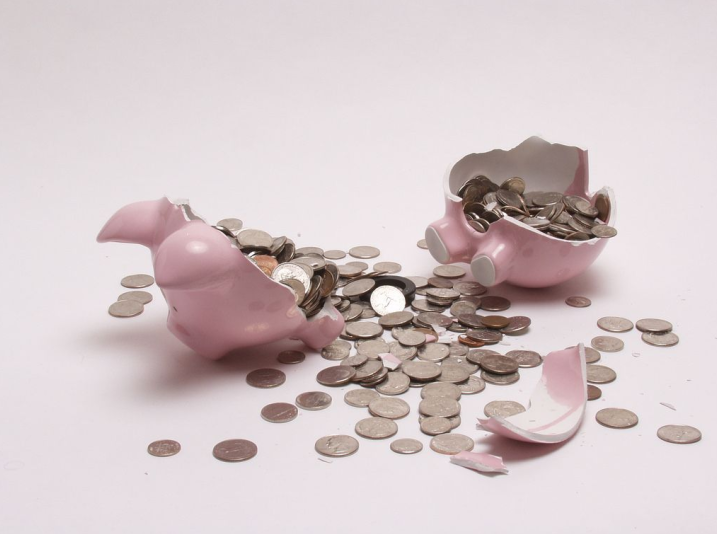
\includegraphics[height=.6\textheight]{Images/tirelire_cassee.png}
\caption{Tout dépenser quand on l'utilise}
\end{figure}
}
\end{block}
\end{frame}

\begin{frame}[label={sec:org4a6cb3d}]{Ça ressemble à quoi une transaction dans un bloc ?}
\begin{block}{Explorons avec l'\href{https://explorer.btc.com/btc/block/772825}{explorer.btc.com}}
\begin{figure}[htbp]
\centering
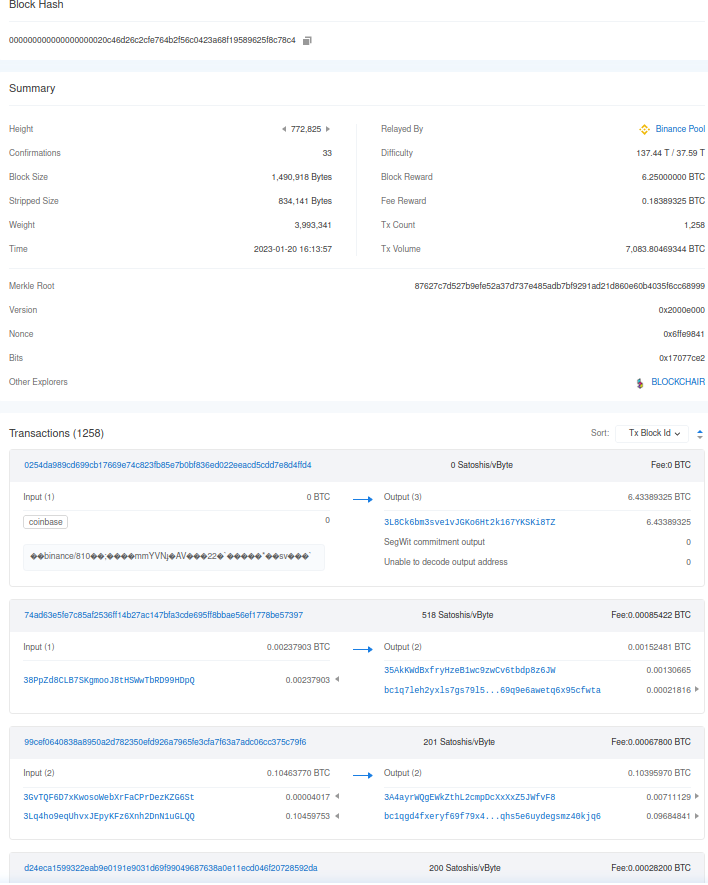
\includegraphics[height=.8\textheight]{Images/binance_bloc.png}
\caption{Un bloc miné hier par Binance}
\end{figure}
\end{block}
\end{frame}


\subsection{Le modèle UTXO plus en détail}
\label{sec:org0e01238}
\begin{frame}<1>[label={sec:orga920807}]{}
\begin{center}
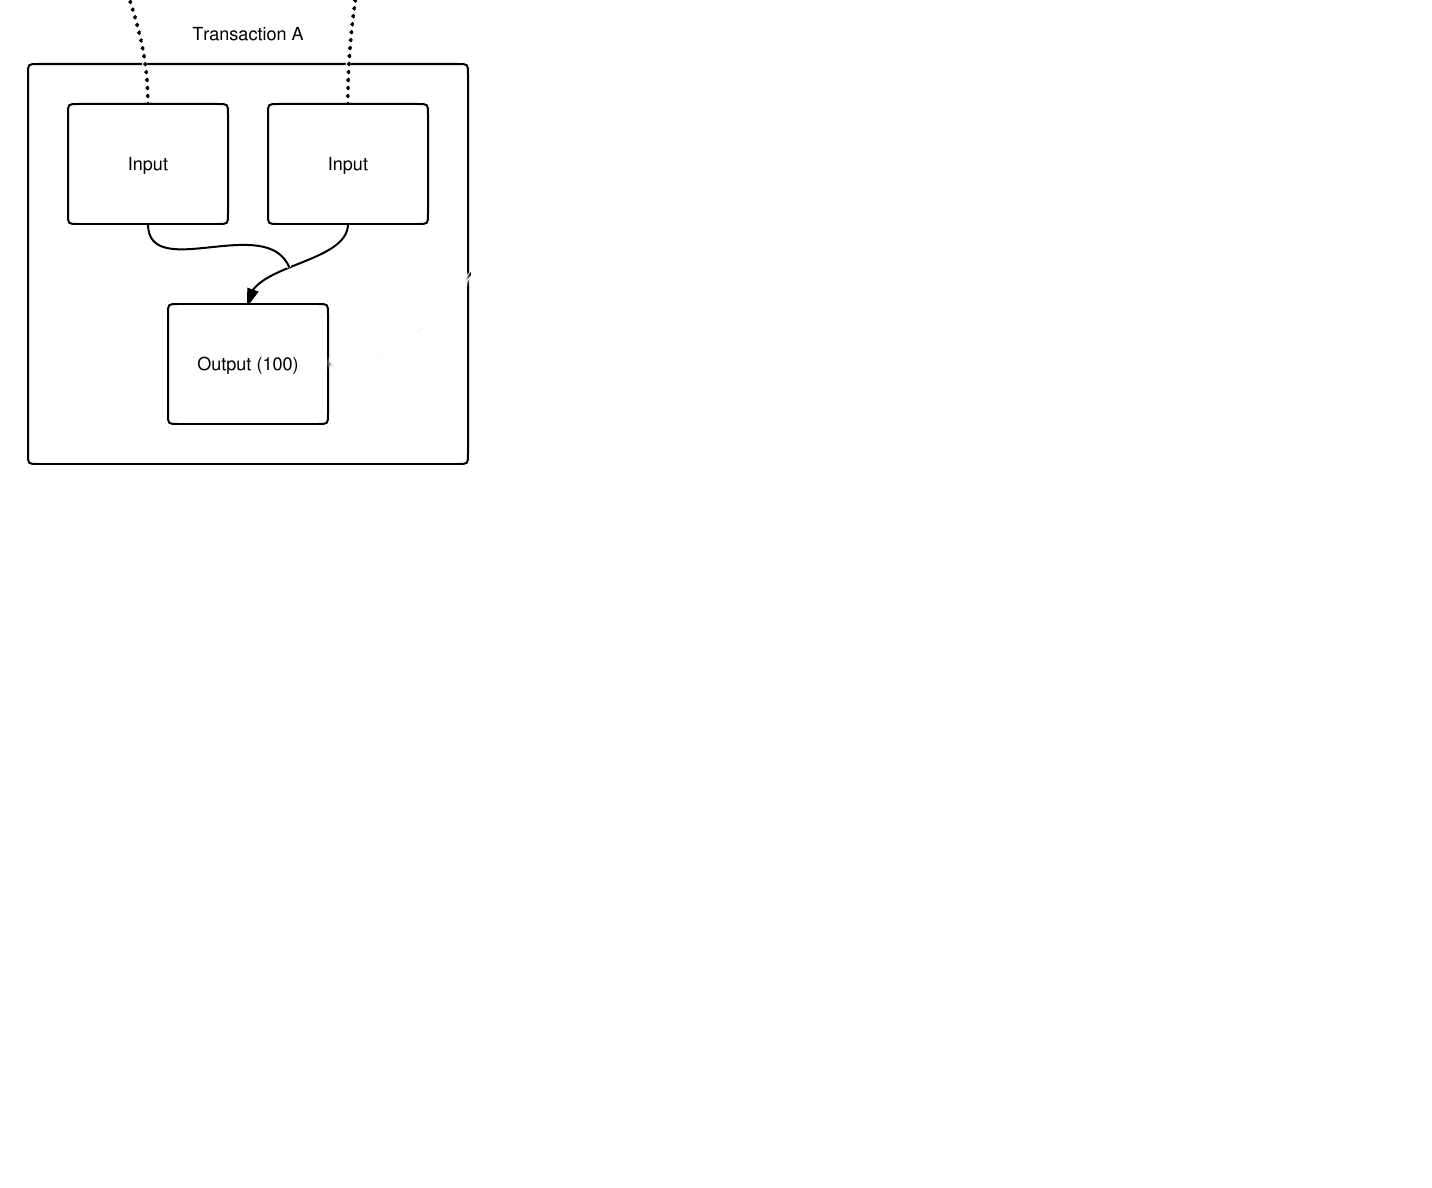
\includegraphics[width=.9\textwidth]{Images/Transaction1.png}
\end{center}
\end{frame}
\begin{frame}<2>[label={sec:org76ab5cc}]{}
\begin{center}
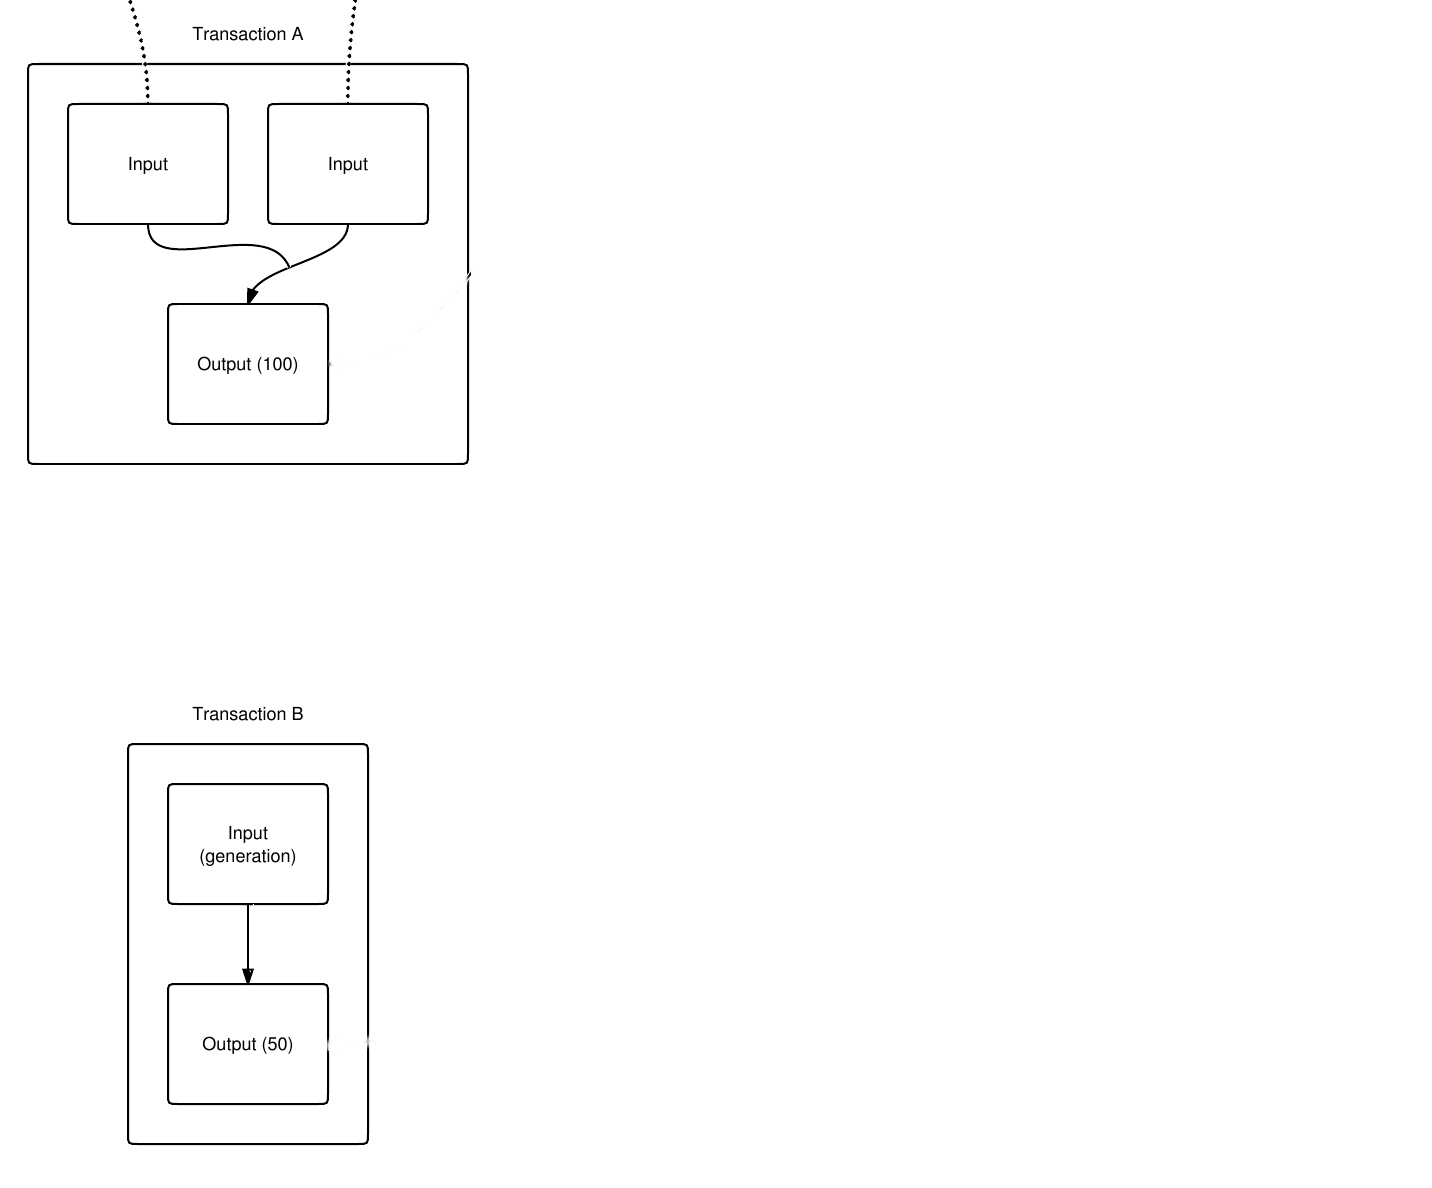
\includegraphics[width=.9\textwidth]{Images/Transaction2.png}
\end{center}
\end{frame}

\begin{frame}<3>[label={sec:org89afbe4}]{}
\begin{center}
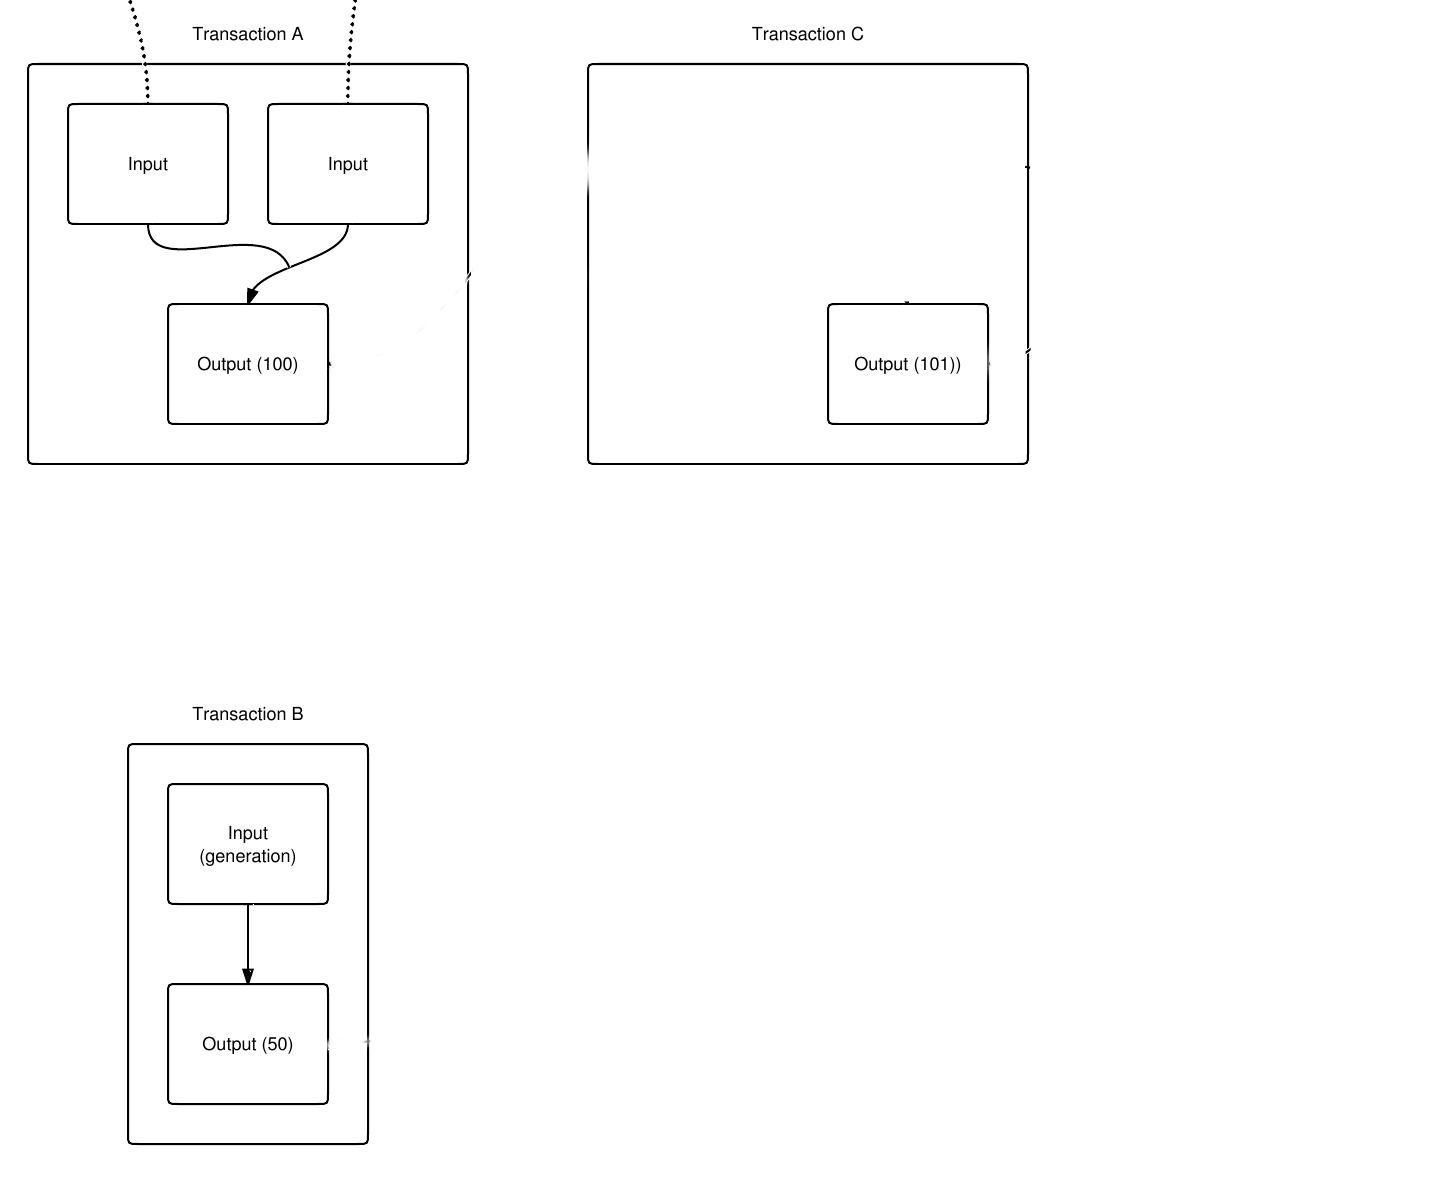
\includegraphics[width=.9\textwidth]{Images/Transaction3.png}
\end{center}
\end{frame}
\begin{frame}<4>[label={sec:org92251a4}]{}
\begin{center}
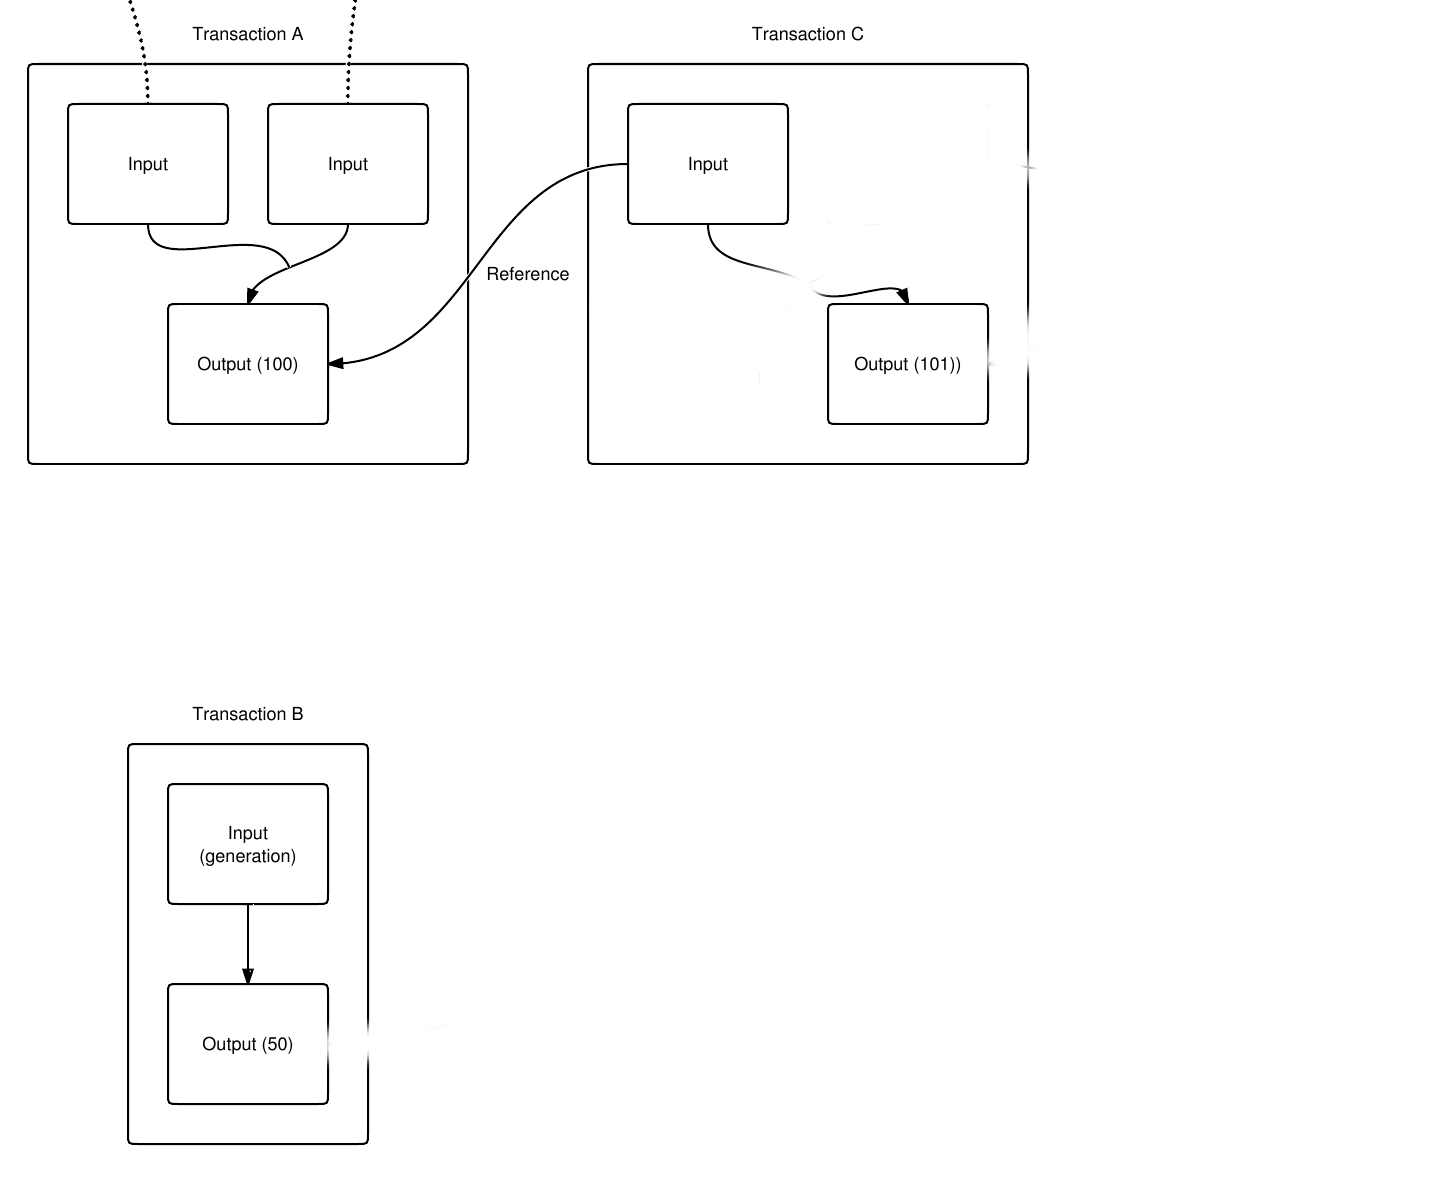
\includegraphics[width=.9\textwidth]{Images/Transaction4.png}
\end{center}
\end{frame}
\begin{frame}<5>[label={sec:orge4d997a}]{}
\begin{center}
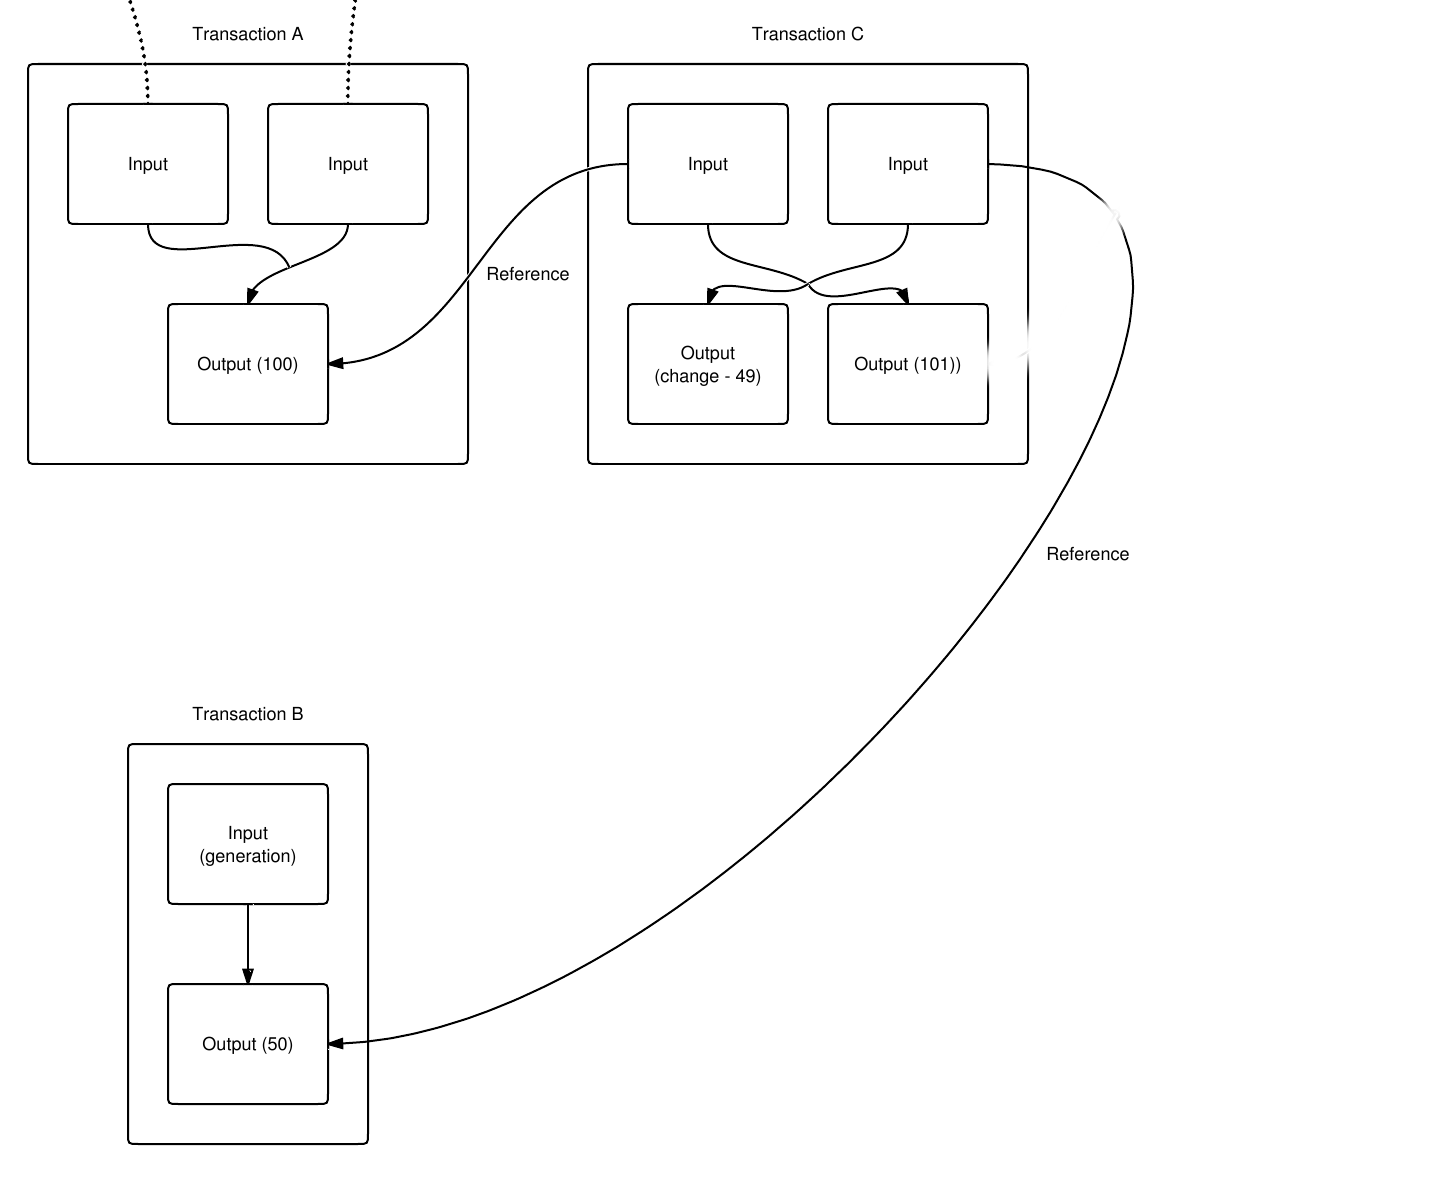
\includegraphics[width=.9\textwidth]{Images/Transaction5.png}
\end{center}
\end{frame}
\begin{frame}<6>[label={sec:org24282c2}]{}
\begin{center}
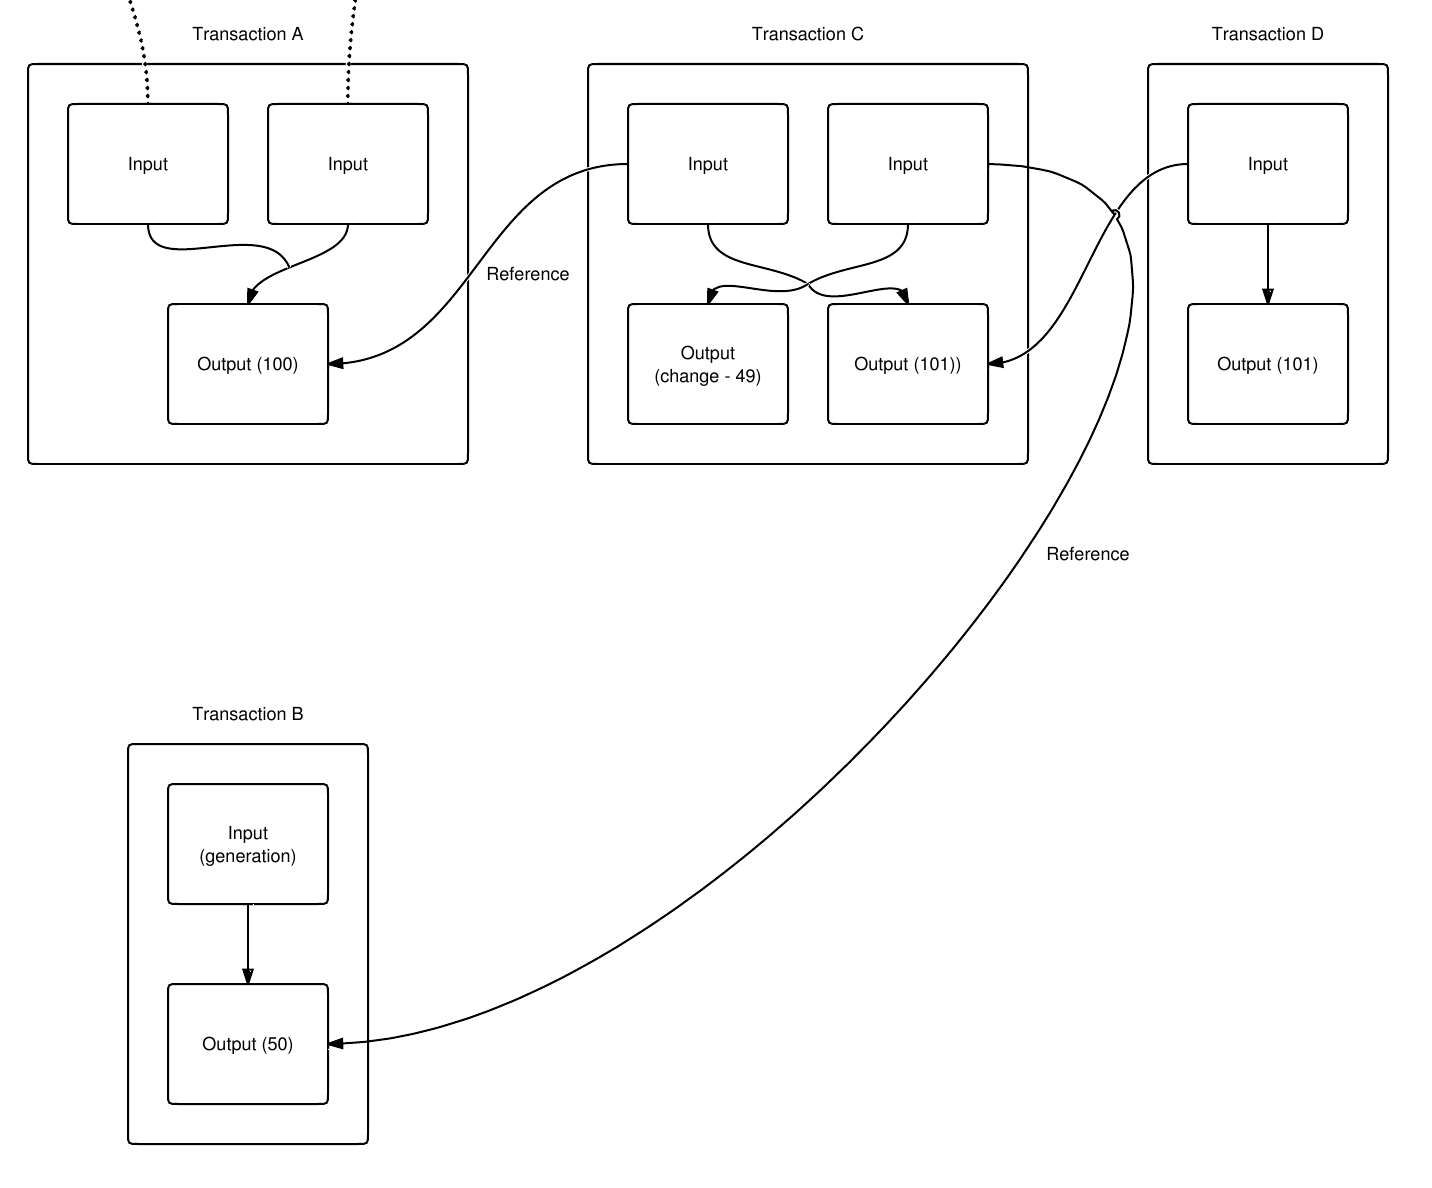
\includegraphics[width=.9\textwidth]{Images/Transaction6.png}
\end{center}
\end{frame}



\begin{frame}[label={sec:org2e9e0eb}]{En résumé}
\begin{itemize}
\item Chaque pièces est unique (non fungible)
\item on réfère des pièces particulières lorsqu'on les dépense
\item les pièces sont consommées et de nouvelles créées
\item on ne peut dépense une pièce qu'une fois.
\end{itemize}
\end{frame}

\subsection{Hash et signatures}
\label{sec:org762f216}
\begin{frame}[label={sec:org3e924b3}]{Propriété des Hash}
\begin{itemize}
\item Résistance à la préimage
\item Résistance à collision
\item impossible de produire la signature d'un autre
\item imposssible de remonter en message en regardant la signature
\item même output pour input identique
\end{itemize}
\begin{block}{SHA256 et RIPEMD160}
quantum resistant
\end{block}
\end{frame}

\subsection{Comment vérifier les transactions}
\label{sec:org517c5b0}
\begin{frame}[label={sec:orgb818462}]{Arbre de Merkle}
\begin{figure}[htbp]
\centering
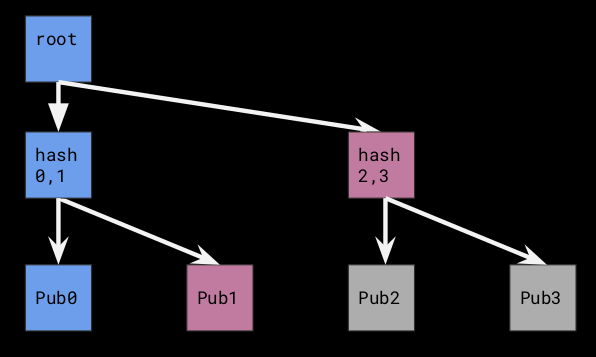
\includegraphics[height=.8\textheight]{Images/merkle.png}
\caption{Arbre de Merkle}
\end{figure}

\begin{itemize}
\item 2500 tx/bloc en moyenne (2019)
\item Prouve qu'une transaction est dans l'arbre rapidement
\end{itemize}
\end{frame}

\subsection{Sécurité des clés}
\label{sec:orgef3aaac}

\begin{frame}[label={sec:org69f860f}]{Création des clefs}
\begin{itemize}
\item La clef privée: un nombre au hasard parmis \(2\textsuperscript{160}\) possibilité
\begin{itemize}
\item environs \(2\textsuperscript{63}\) grains de sable sur terre
\item Chance d'avoir le même grain de sable <0.0001$\backslash$%
\item Il y a des milliard de milliards d'adresses pour tous les humains
\end{itemize}
\item La clef publique, générée à partir de la clef privée
\item Les addresses publiques sont générées à partir de la clef publique
\end{itemize}
\end{frame}

\begin{frame}[label={sec:org48fb07c}]{ECDSA elipitic Curve Digital Signature Algorithm}
\begin{columns}
\begin{column}{0.46\columnwidth}
\begin{block}<1->{Génération des clés}
\begin{itemize}
\item Si on connait P et Q -> R
\item Mais R ne permet pas de trouver P et Q
\end{itemize}
\end{block}
\end{column}

\begin{column}{0.46\columnwidth}
\begin{block}<1->{}
\begin{figure}[htbp]
\centering
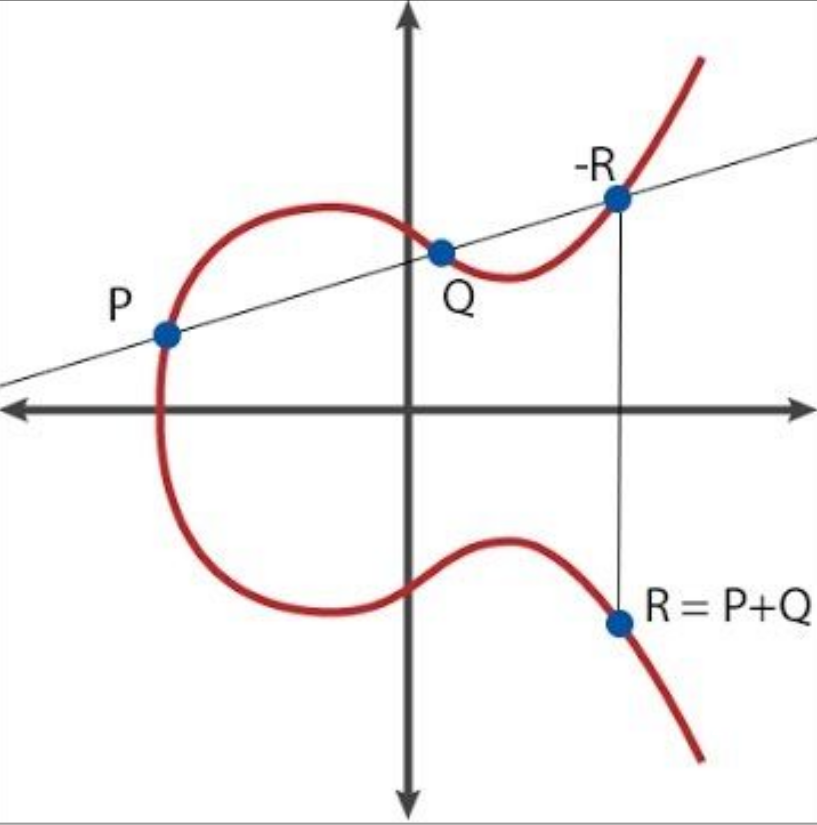
\includegraphics[width=.8\textwidth]{Images/eliptic.png}
\caption{Courbe eliptic \(y^2 = x^3 +7\)}
\end{figure}
\end{block}
\end{column}
\end{columns}
\end{frame}



\section{Systèmes distribués}
\label{sec:org5091e83}
\subsection{Système distrivués}
\label{sec:orgaf3e8dd}
\begin{frame}[label={sec:org5a1062d}]{De l'infiniment petit à l'infiniment grand}
\begin{center}
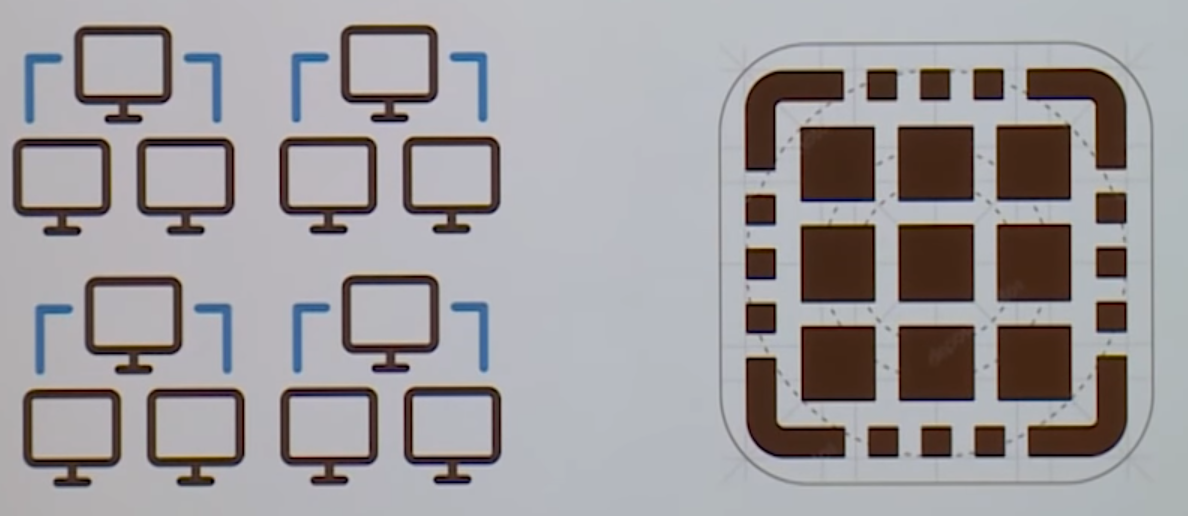
\includegraphics[width=.6\textwidth]{Images/grand_petit.png}
\end{center}

\begin{columns}
\begin{column}{0.46\columnwidth}
\begin{block}<1->{Petit}
\begin{figure}[htbp]
\centering
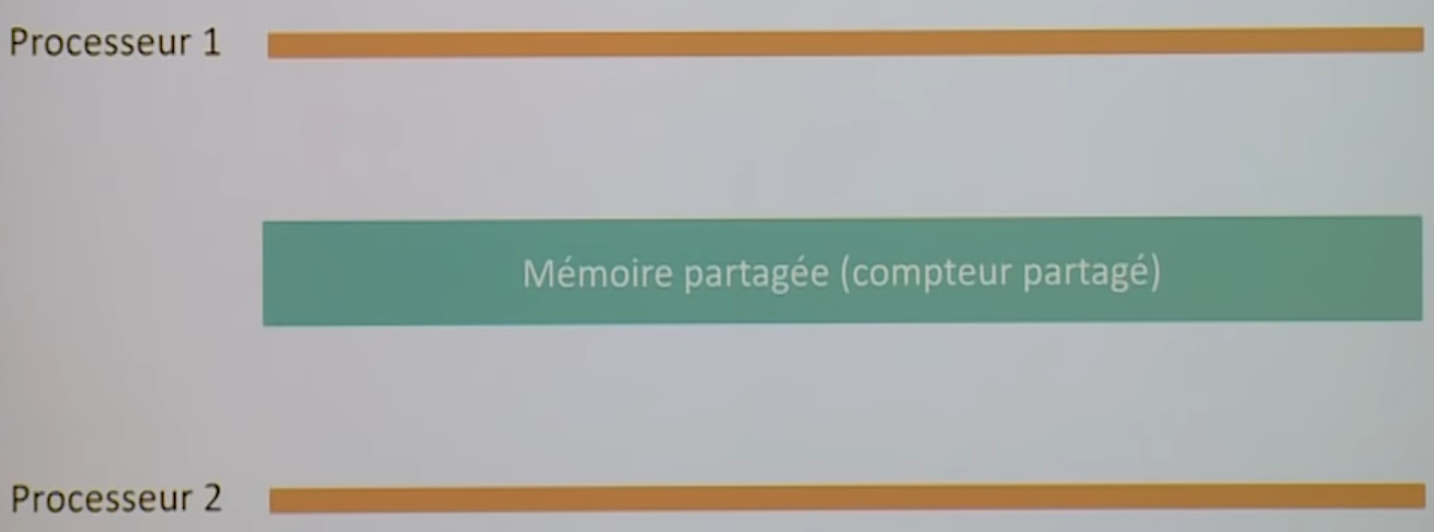
\includegraphics[width=.8\textwidth]{Images/memoire_partagee.png}
\caption{Avec memoire partagé}
\end{figure}
\end{block}
\end{column}


\begin{column}{0.46\columnwidth}
\begin{block}<1->{Grand}
\begin{figure}[htbp]
\centering
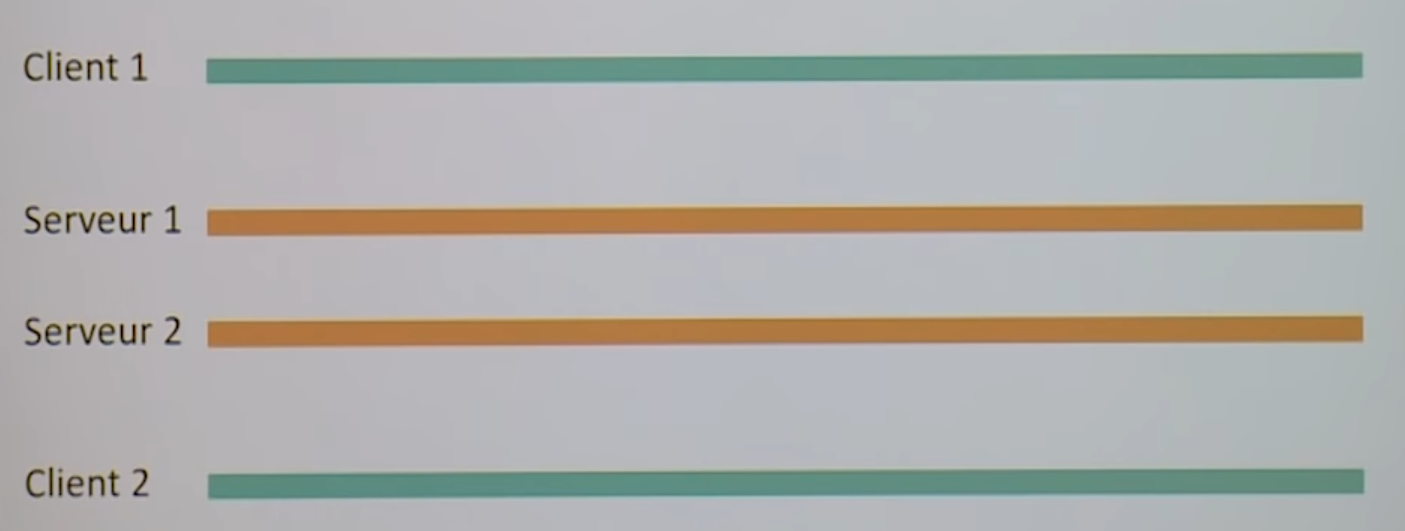
\includegraphics[width=.8\textwidth]{Images/envoi_message.png}
\caption{Avec envois de messages}
\end{figure}
\end{block}
\end{column}
\end{columns}
\end{frame}



\begin{frame}[label={sec:orgb3001bc}]{Propriétés des Systèmes distribués}
\begin{columns}
\begin{column}{0.46\columnwidth}
\begin{block}{}
\begin{itemize}
\item <1-> \alert{Robustesse} :  la machine fonctionne toujours
\item <2> \alert{Atomocite} : elle est perçu comme une seule machine
\end{itemize}
\end{block}
\end{column}

\begin{column}{0.46\columnwidth}
\begin{block}<2>{}
\only<1>{
\begin{center}
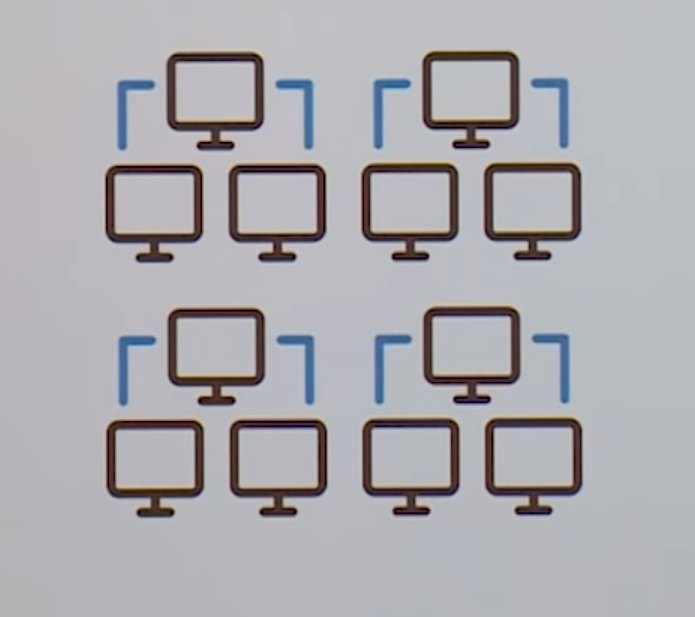
\includegraphics[width=.8\textwidth]{Images/robuste.png}
\end{center}

}

\only<2>{          
\begin{center}
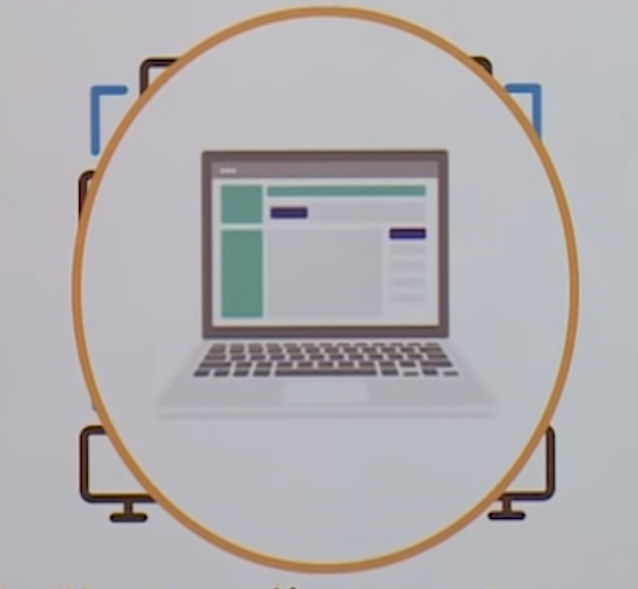
\includegraphics[width=.8\textwidth]{Images/atomicite.png}
\end{center}
}
\end{block}
\end{column}
\end{columns}
\end{frame}

\begin{frame}[label={sec:orgb2a19c2}]{Problèmes des Systèmes distribués}
\begin{columns}
\begin{column}{0.60\columnwidth}
\begin{block}{}
\begin{itemize}
\item <1> Complexité
\item <2> Perte de \alert{l'universalité}
\end{itemize}
\begin{block}{}
\only<2>{
Tout ce qui \emph{était} calculable l'était avec la \alert{Machine de Turing}
}
\end{block}
\end{block}
\end{column}

\begin{column}{0.40\columnwidth}
\begin{block}{}
\only<1>{
\begin{center}
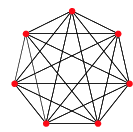
\includegraphics[width=\textwidth]{Images/graphe_complexe.png}
\end{center}
}
\only<2>{
\begin{center}
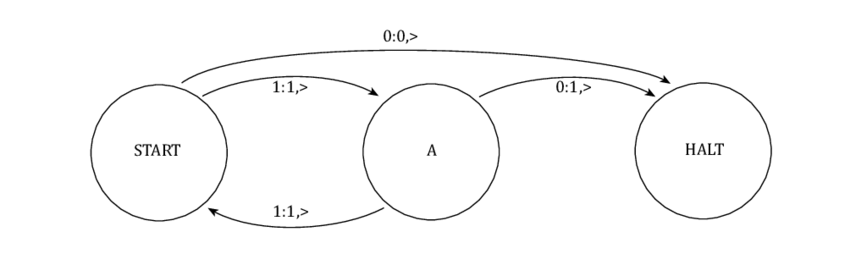
\includegraphics[width=\textwidth]{Images/turing_schema.png}
\end{center}
}
\end{block}
\end{column}
\end{columns}
\end{frame}


\subsection{Les Généraux Byzantins}
\label{sec:org017b24c}
\begin{frame}[label={sec:org09c9e6c}]{Attaque ou retraite ?}
\begin{block}{Le problème des généraux Byzantins}
\only<1>{
\begin{figure}[htbp]
\centering
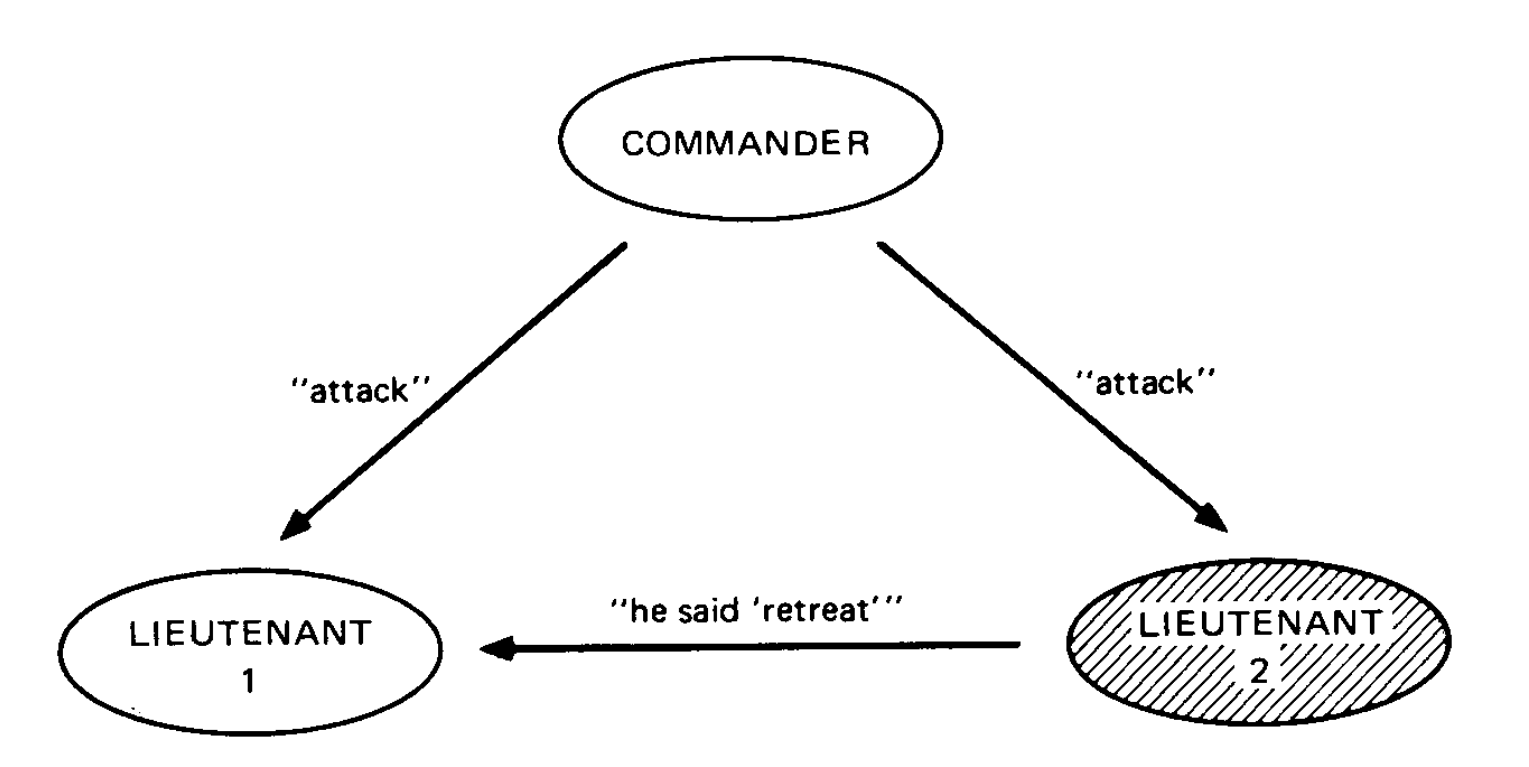
\includegraphics[width=.9\textwidth]{Images/byzantine_gp1.png}
\caption{Le lieutenant est un traitre}
\end{figure}
}

\only<2>{
\begin{figure}[htbp]
\centering
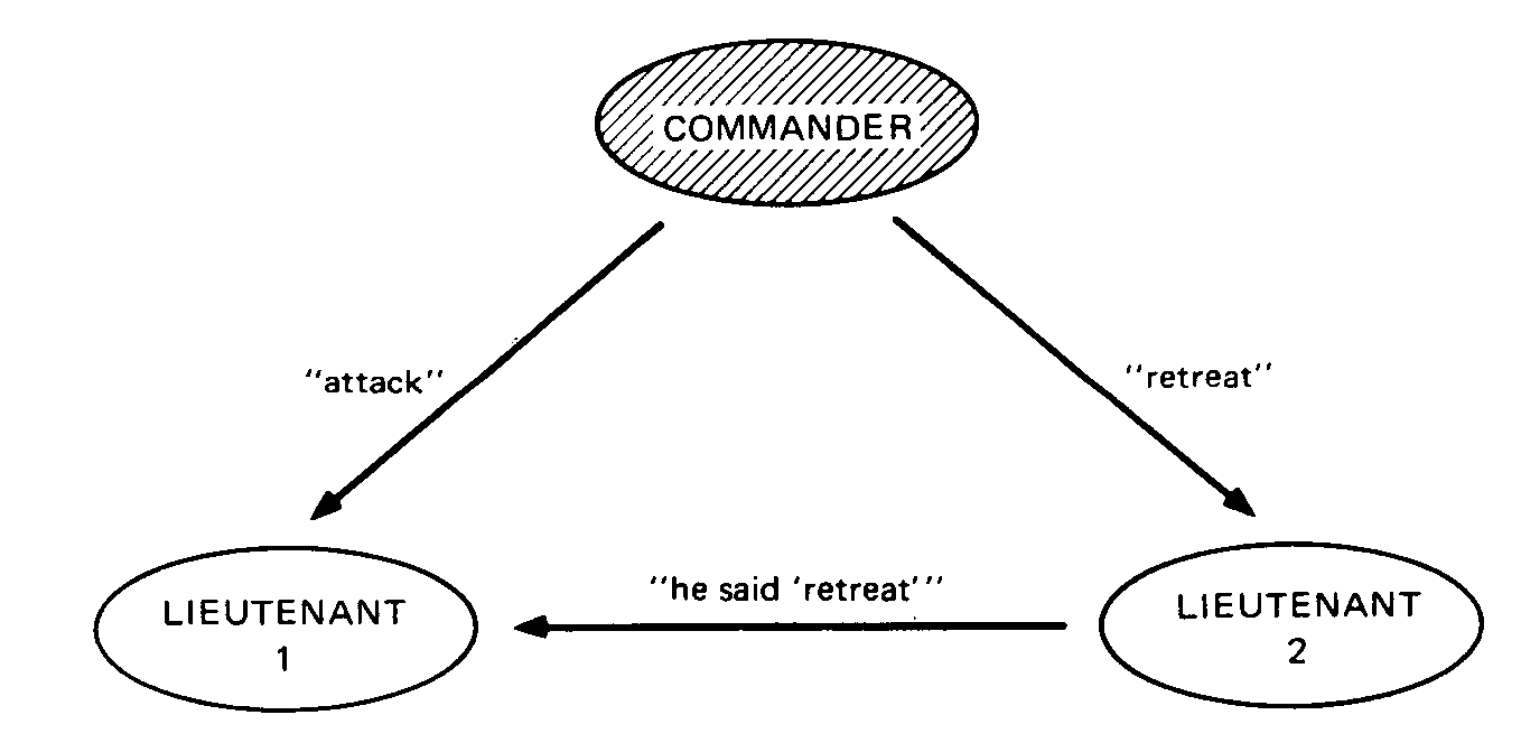
\includegraphics[width=.9\textwidth]{Images/byzantine_gp2.png}
\caption{Le commandant est un traitre}
\end{figure}
}
\end{block}
\end{frame}

\begin{frame}[label={sec:org9294e01}]{BFT Systems}
\begin{block}{\emph{Systèmes tolérants aux fautes Byzantines}}
\begin{itemize}
\item Nombre et participants connus
\item Election d'un leader
\item Traites Punis
\end{itemize}

\begin{block}{Sans signature}
\begin{itemize}
\item honnête majorité obligatoire
\end{itemize}
\end{block}
\begin{block}{Avec signature}
\begin{itemize}
\item Pas de majorité obligatoire
\end{itemize}
\end{block}
\end{block}
\end{frame}

\subsection{Blockchains et consensus}
\label{sec:orgb9218ee}
\begin{frame}[label={sec:orgf49b2d8}]{Preuve de travail (PoW) : Consensus de Nakamoto}
\only<1>{
\begin{center}
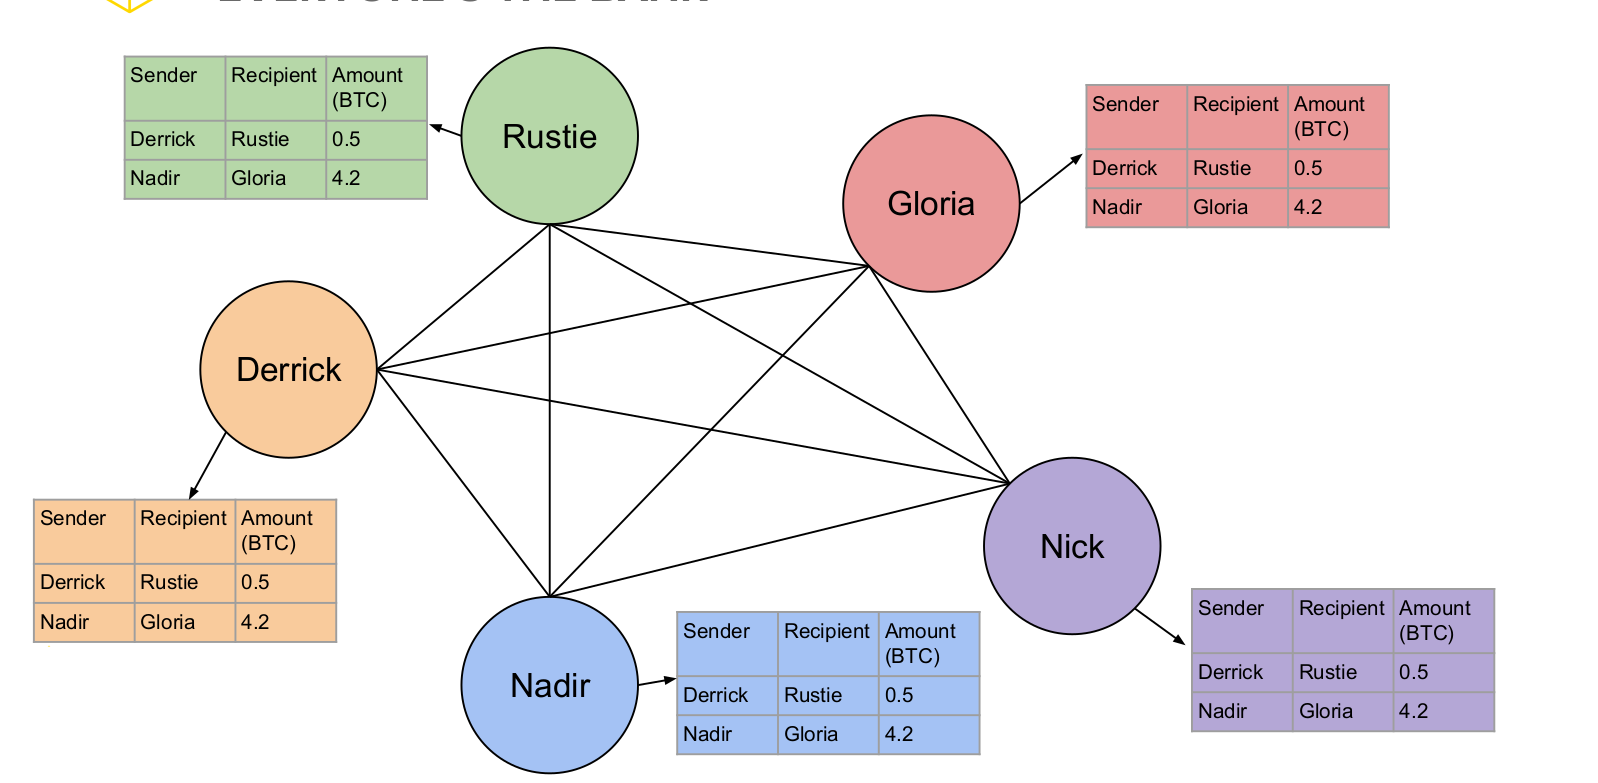
\includegraphics[height=.8\textheight]{Images/distrib2.png}
\end{center}
}

\only<2>{
\begin{center}
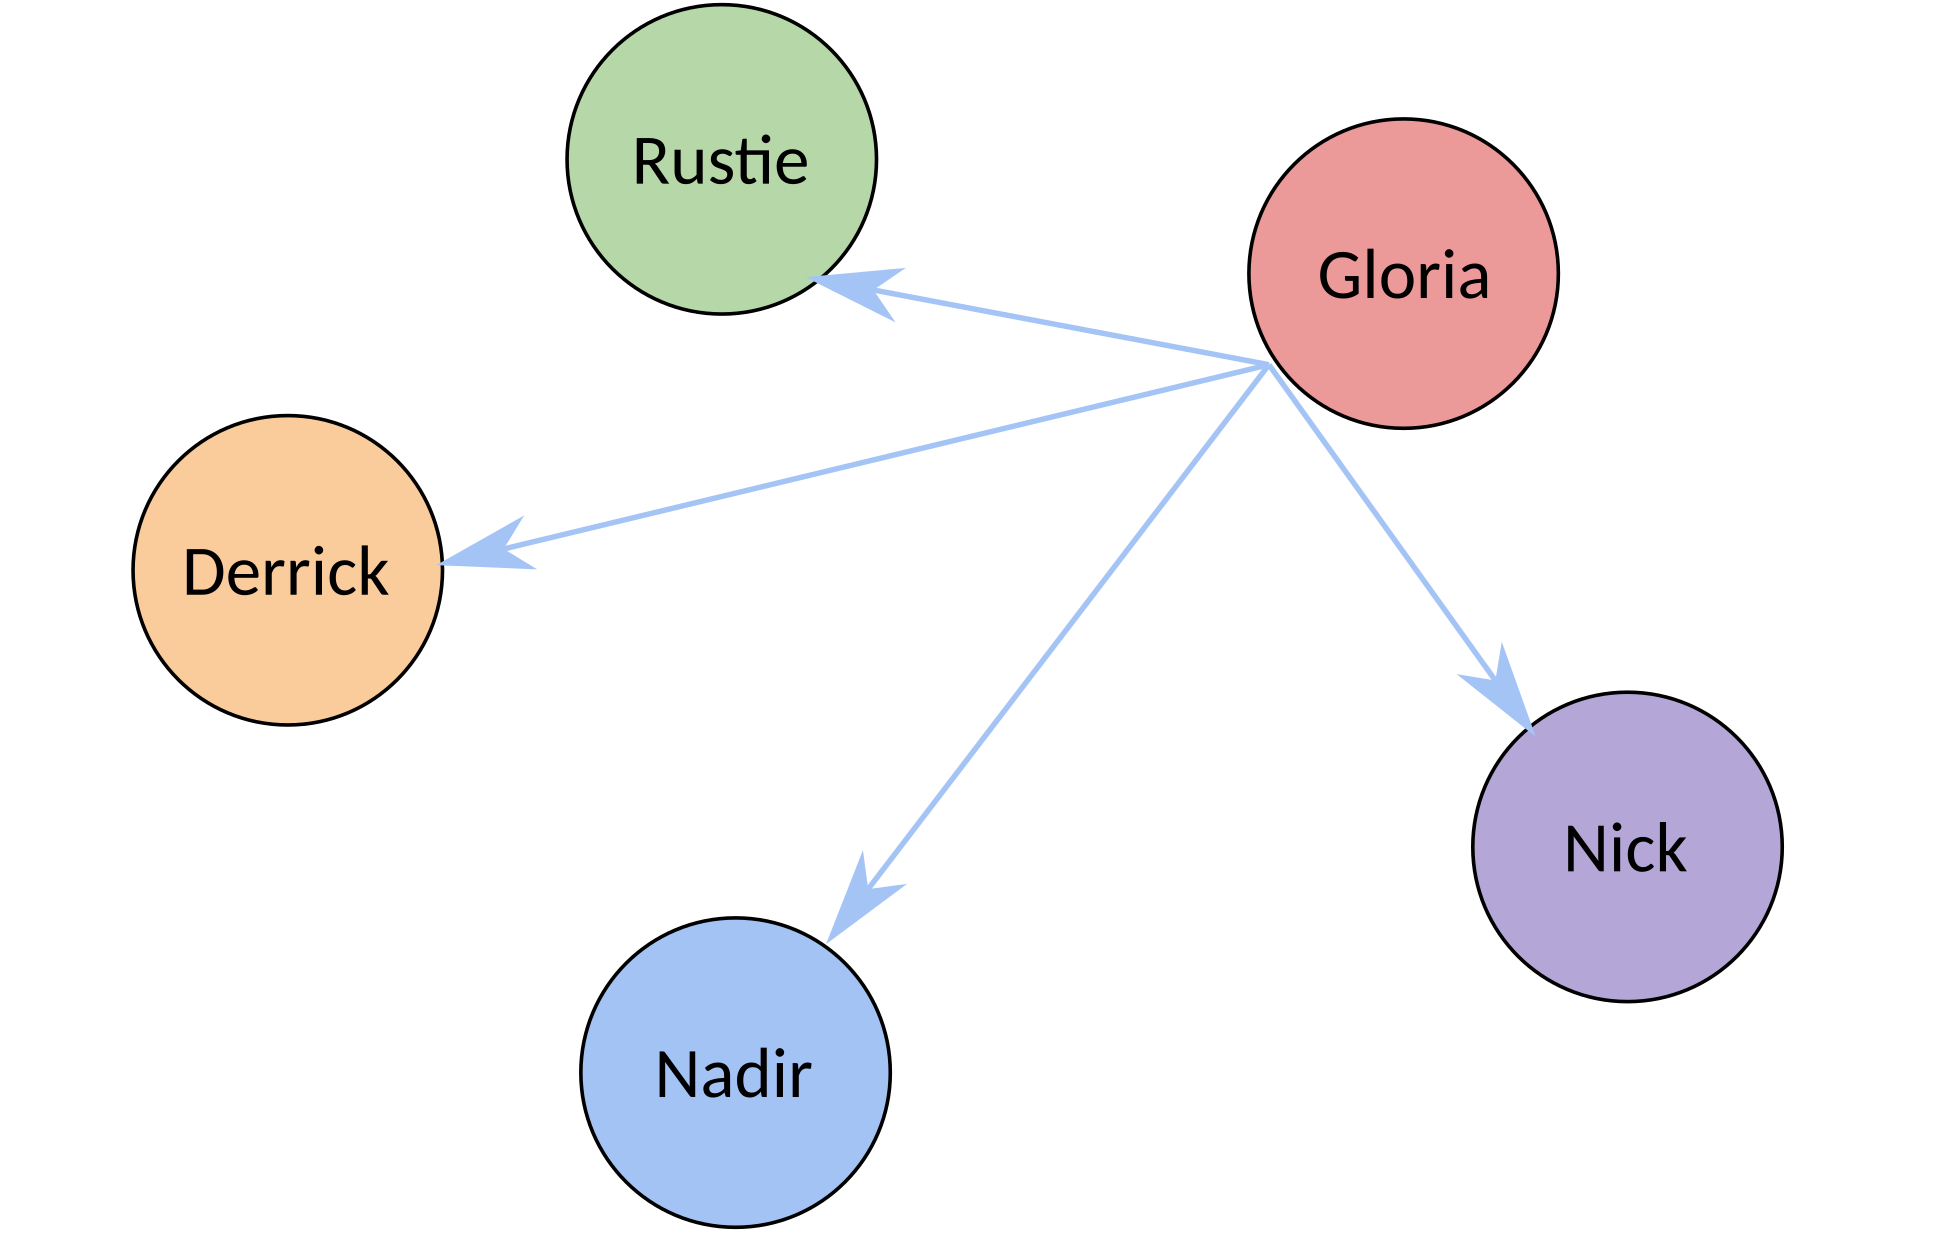
\includegraphics[height=.8\textheight]{Images/consensus1.png}
\end{center}
}

\only<3>{
\begin{center}
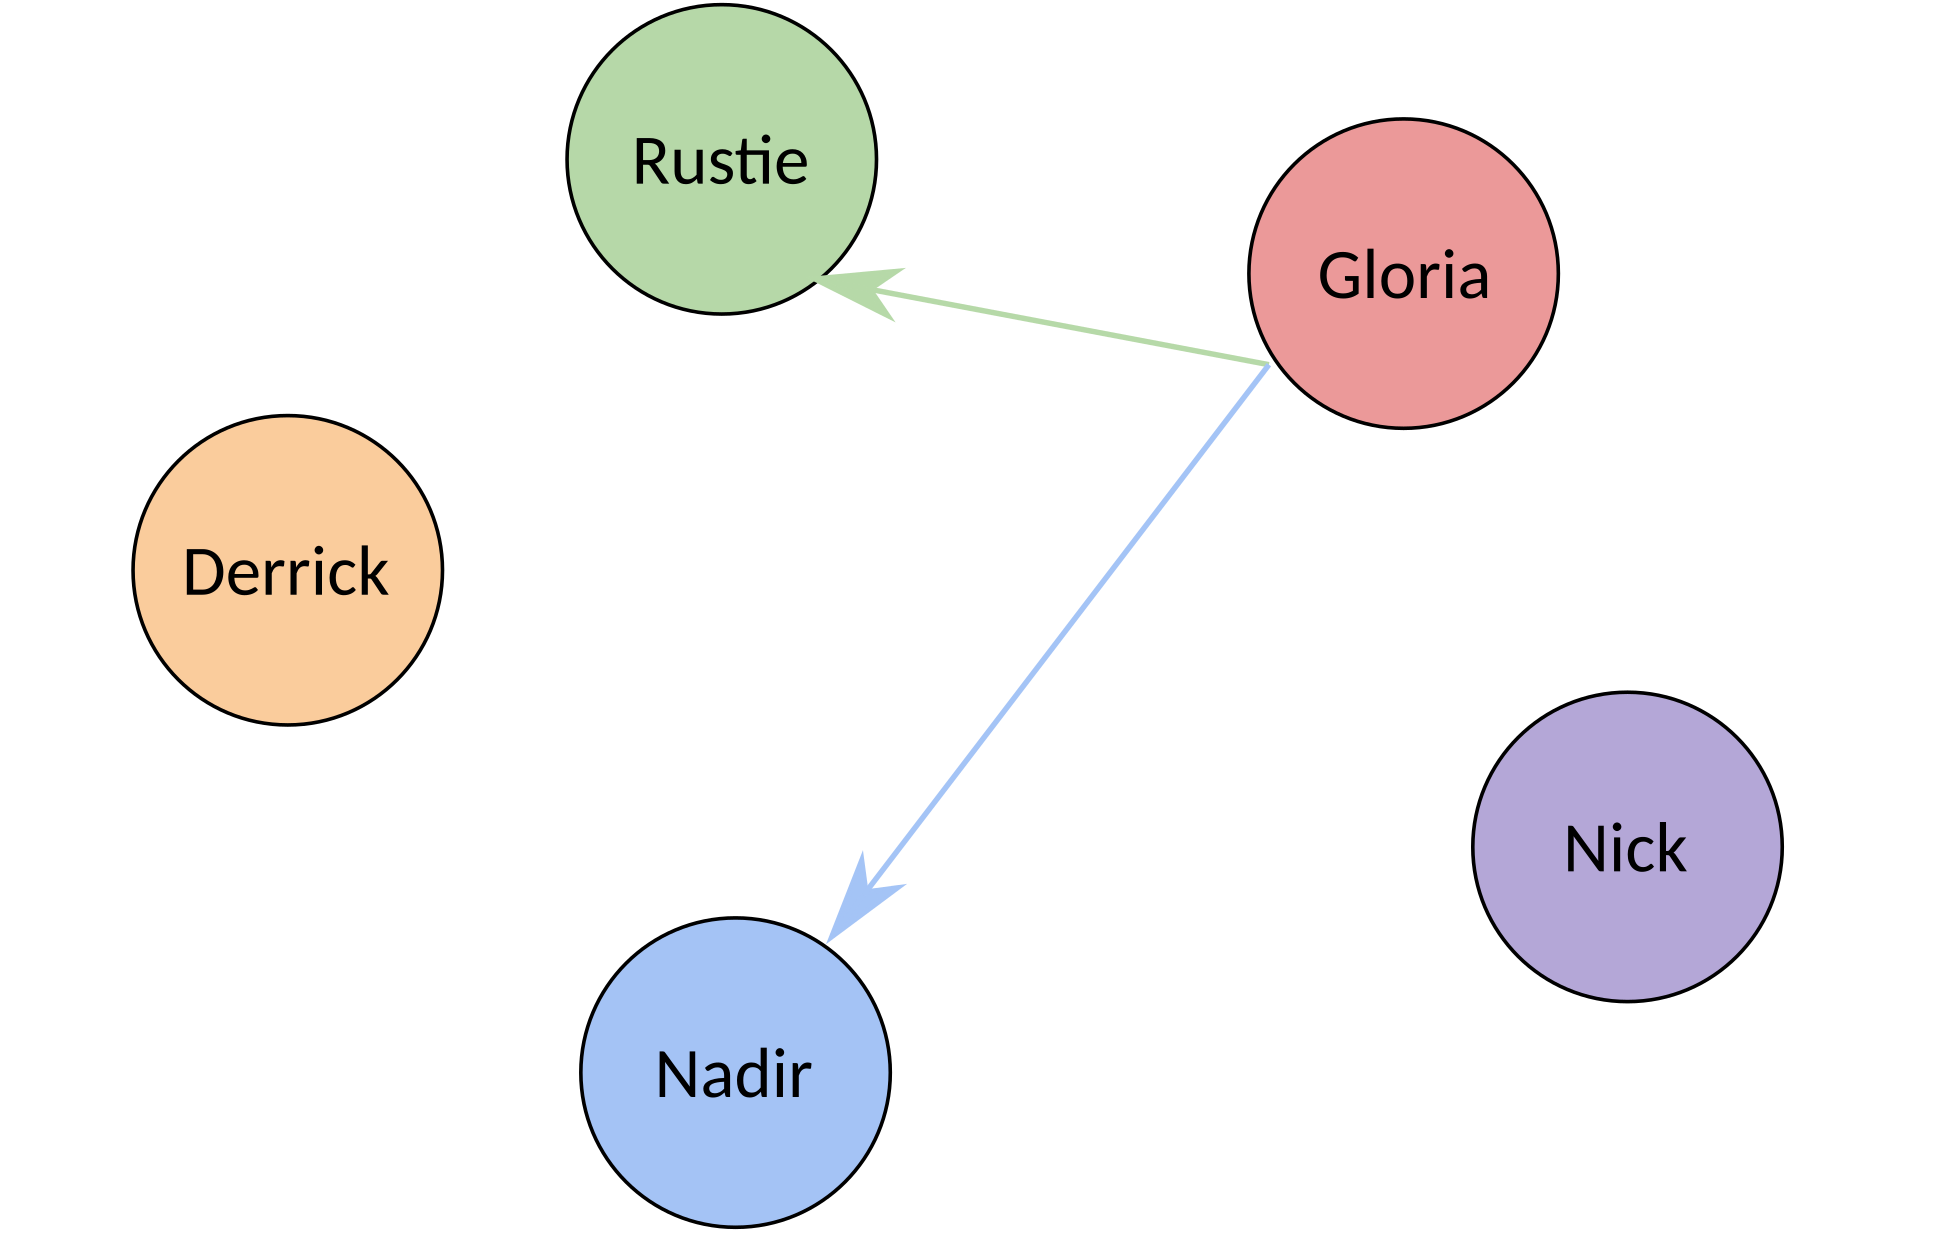
\includegraphics[height=.8\textheight]{Images/consensus2.png}
\end{center}
}
\only<4>{
\begin{center}
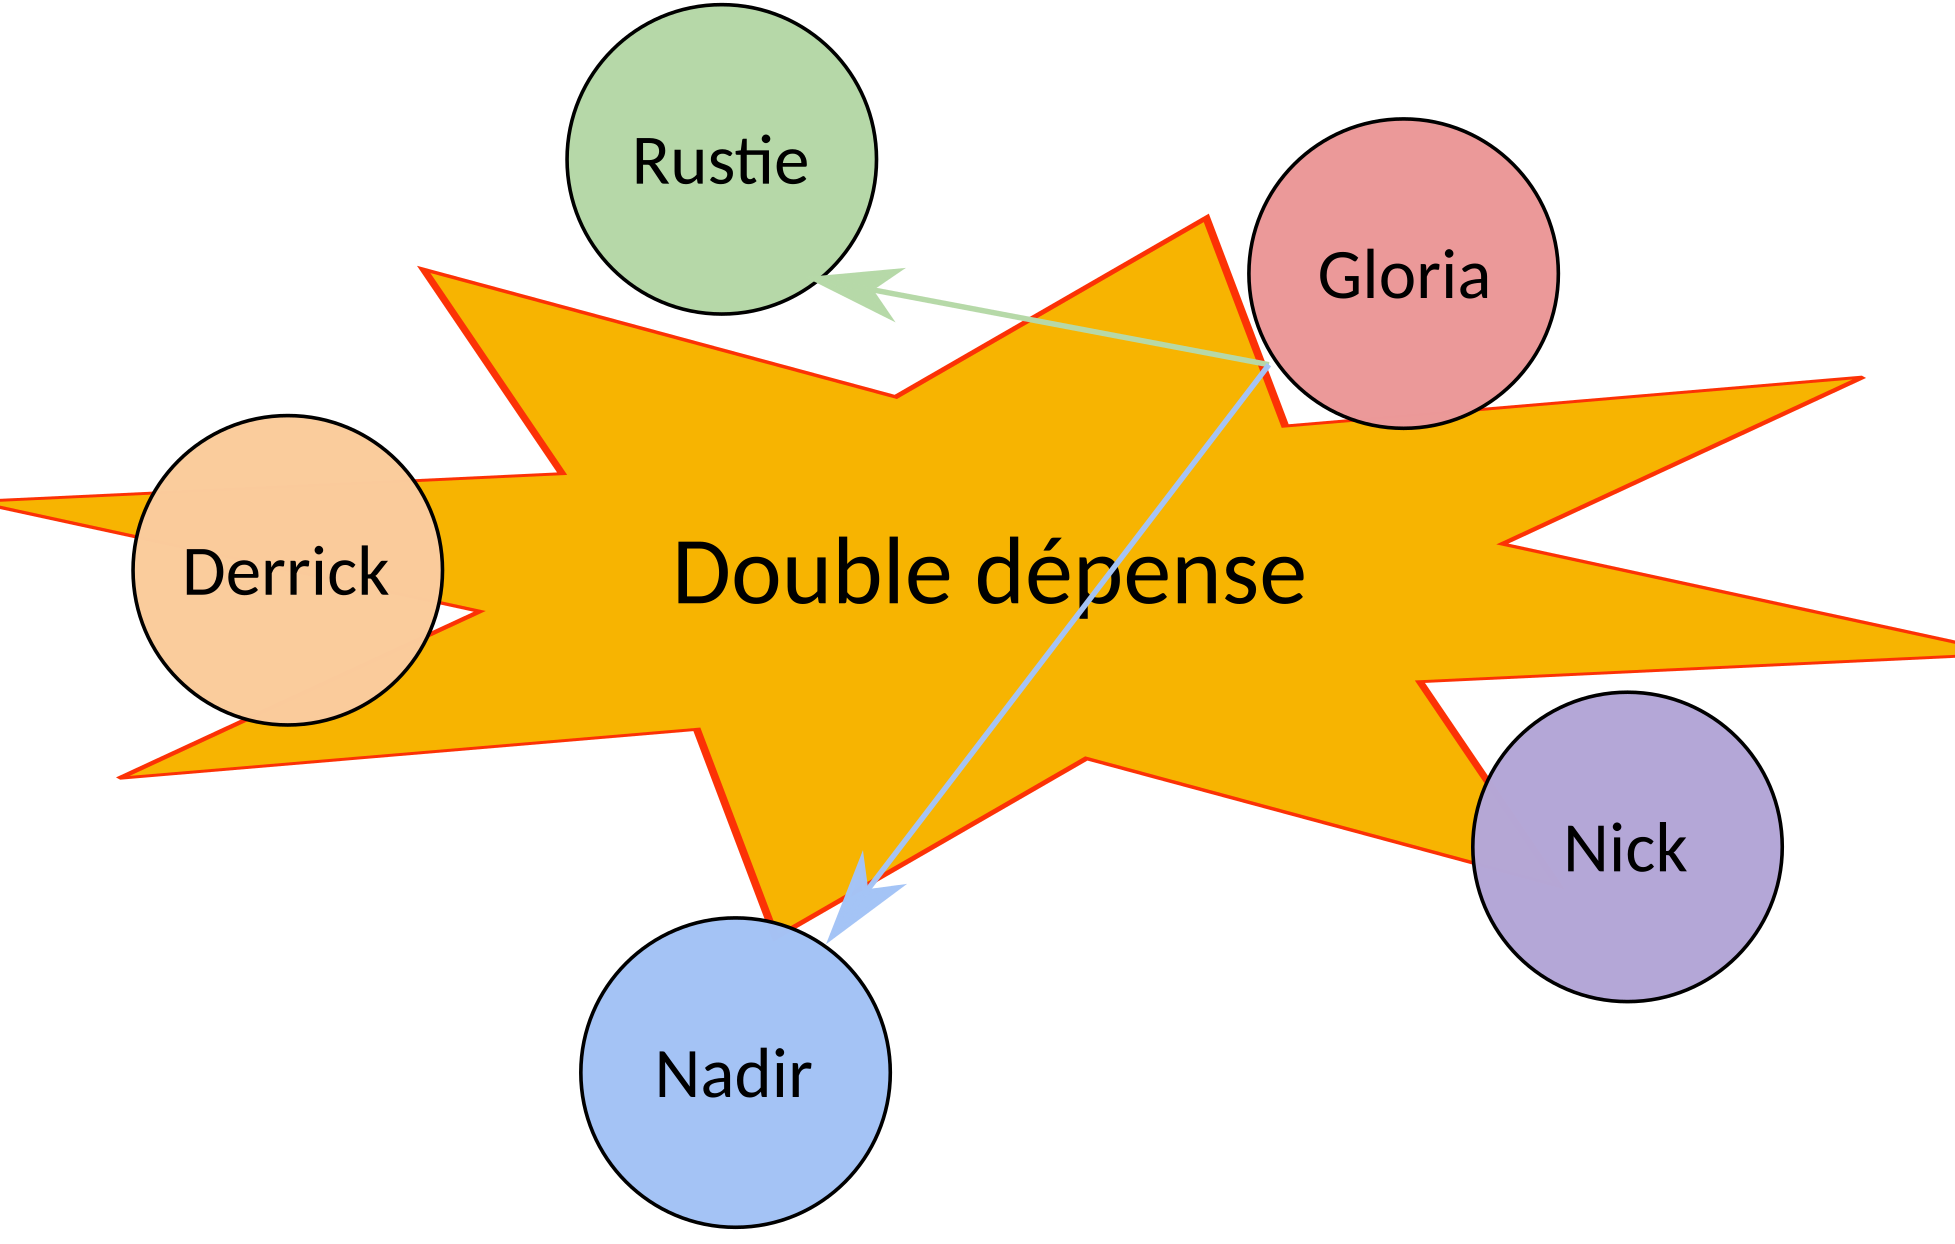
\includegraphics[height=.8\textheight]{Images/consensus3.png}
\end{center}
}
\only<5>{
\begin{center}
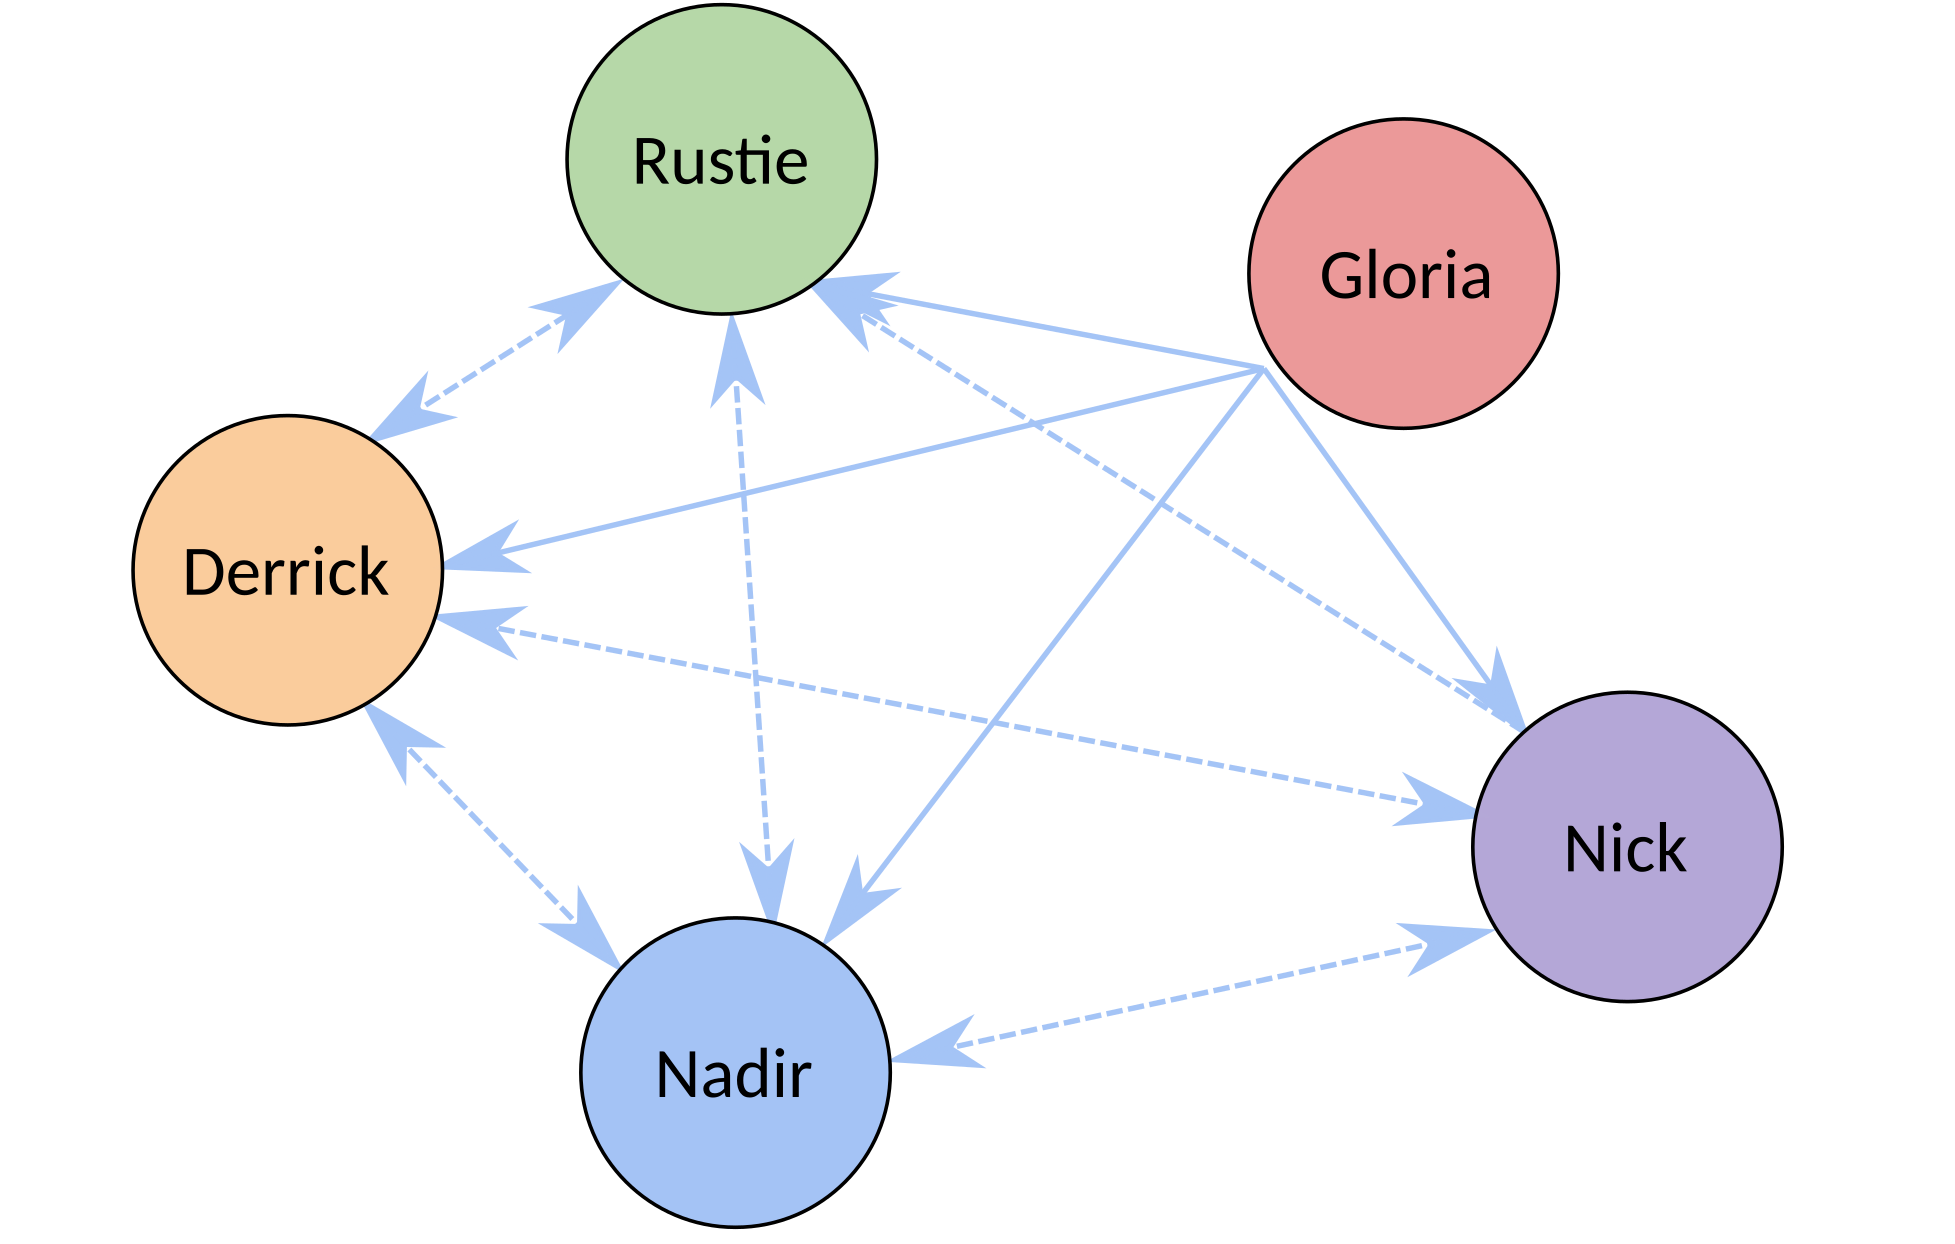
\includegraphics[height=.8\textheight]{Images/consensus4.png}
\end{center}
}
\only<6>{
\begin{center}
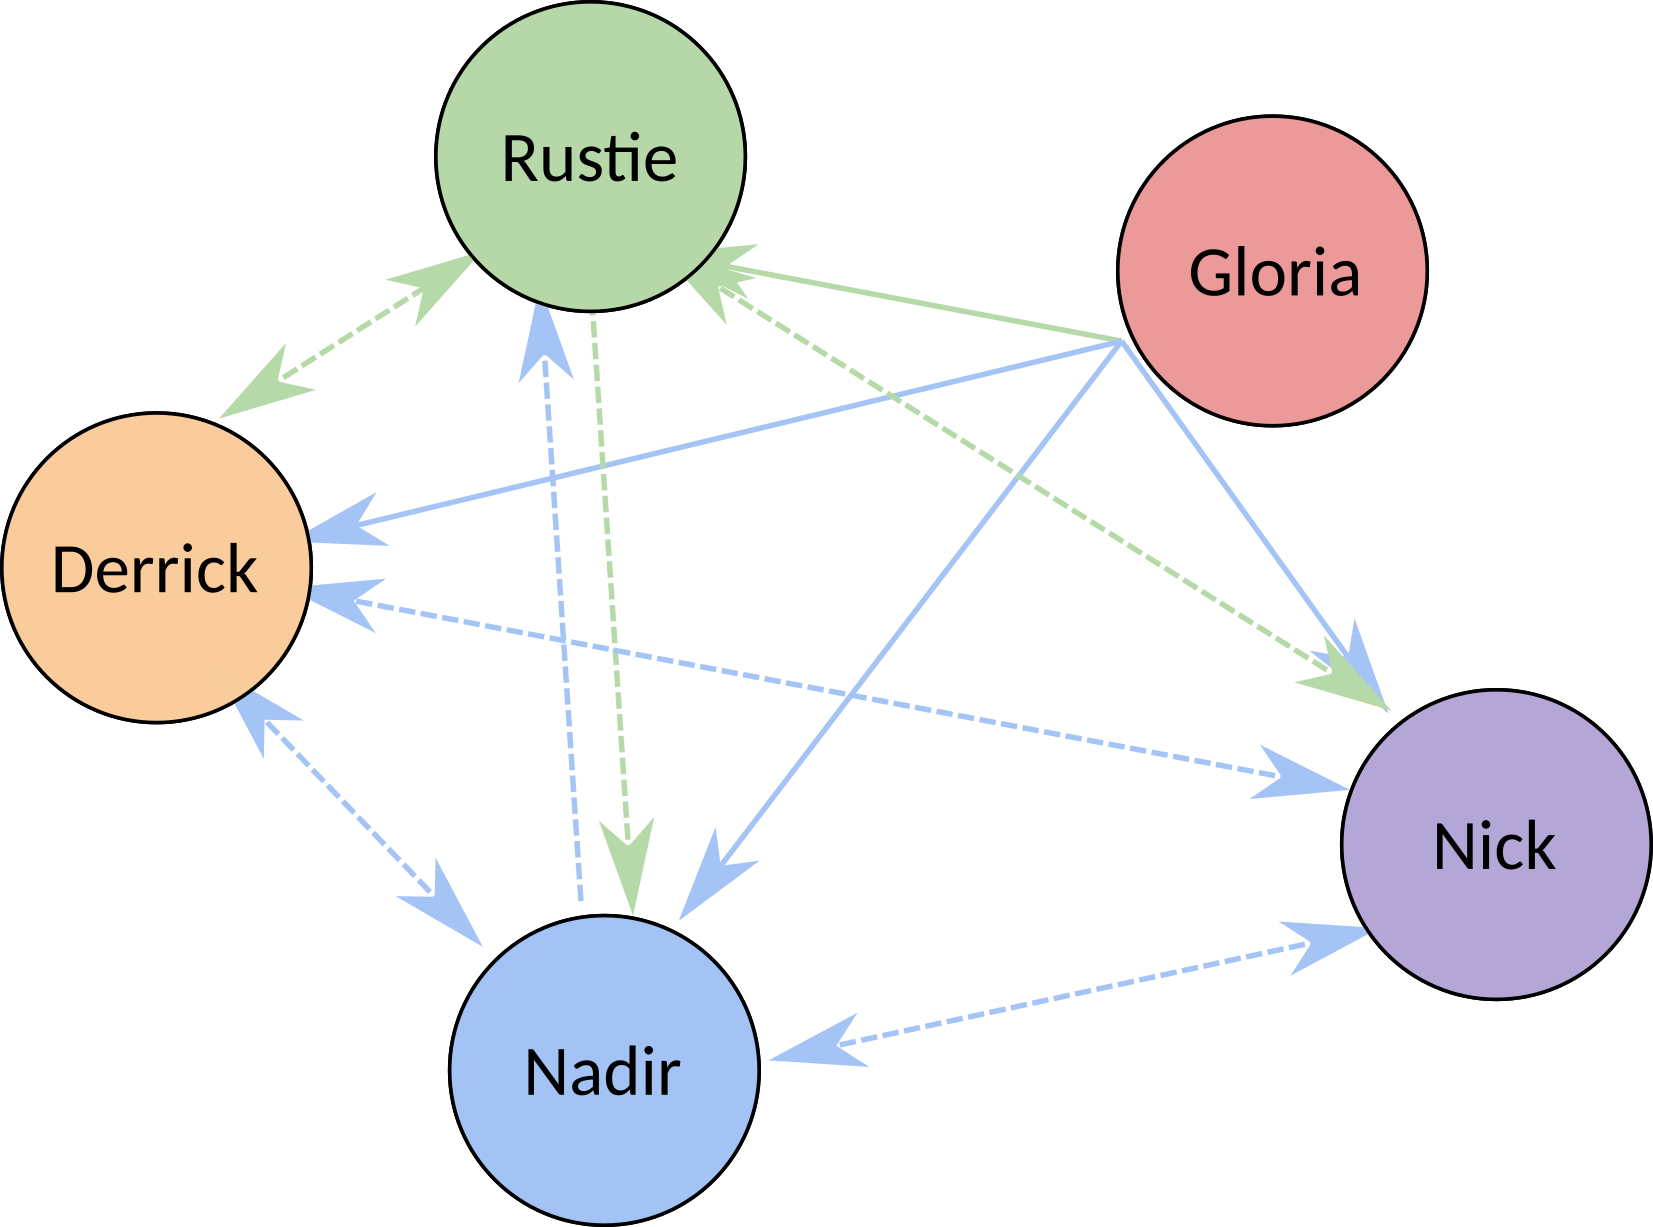
\includegraphics[height=.8\textheight]{Images/consensus5.png}
\end{center}
}
\only<7>{
\begin{center}
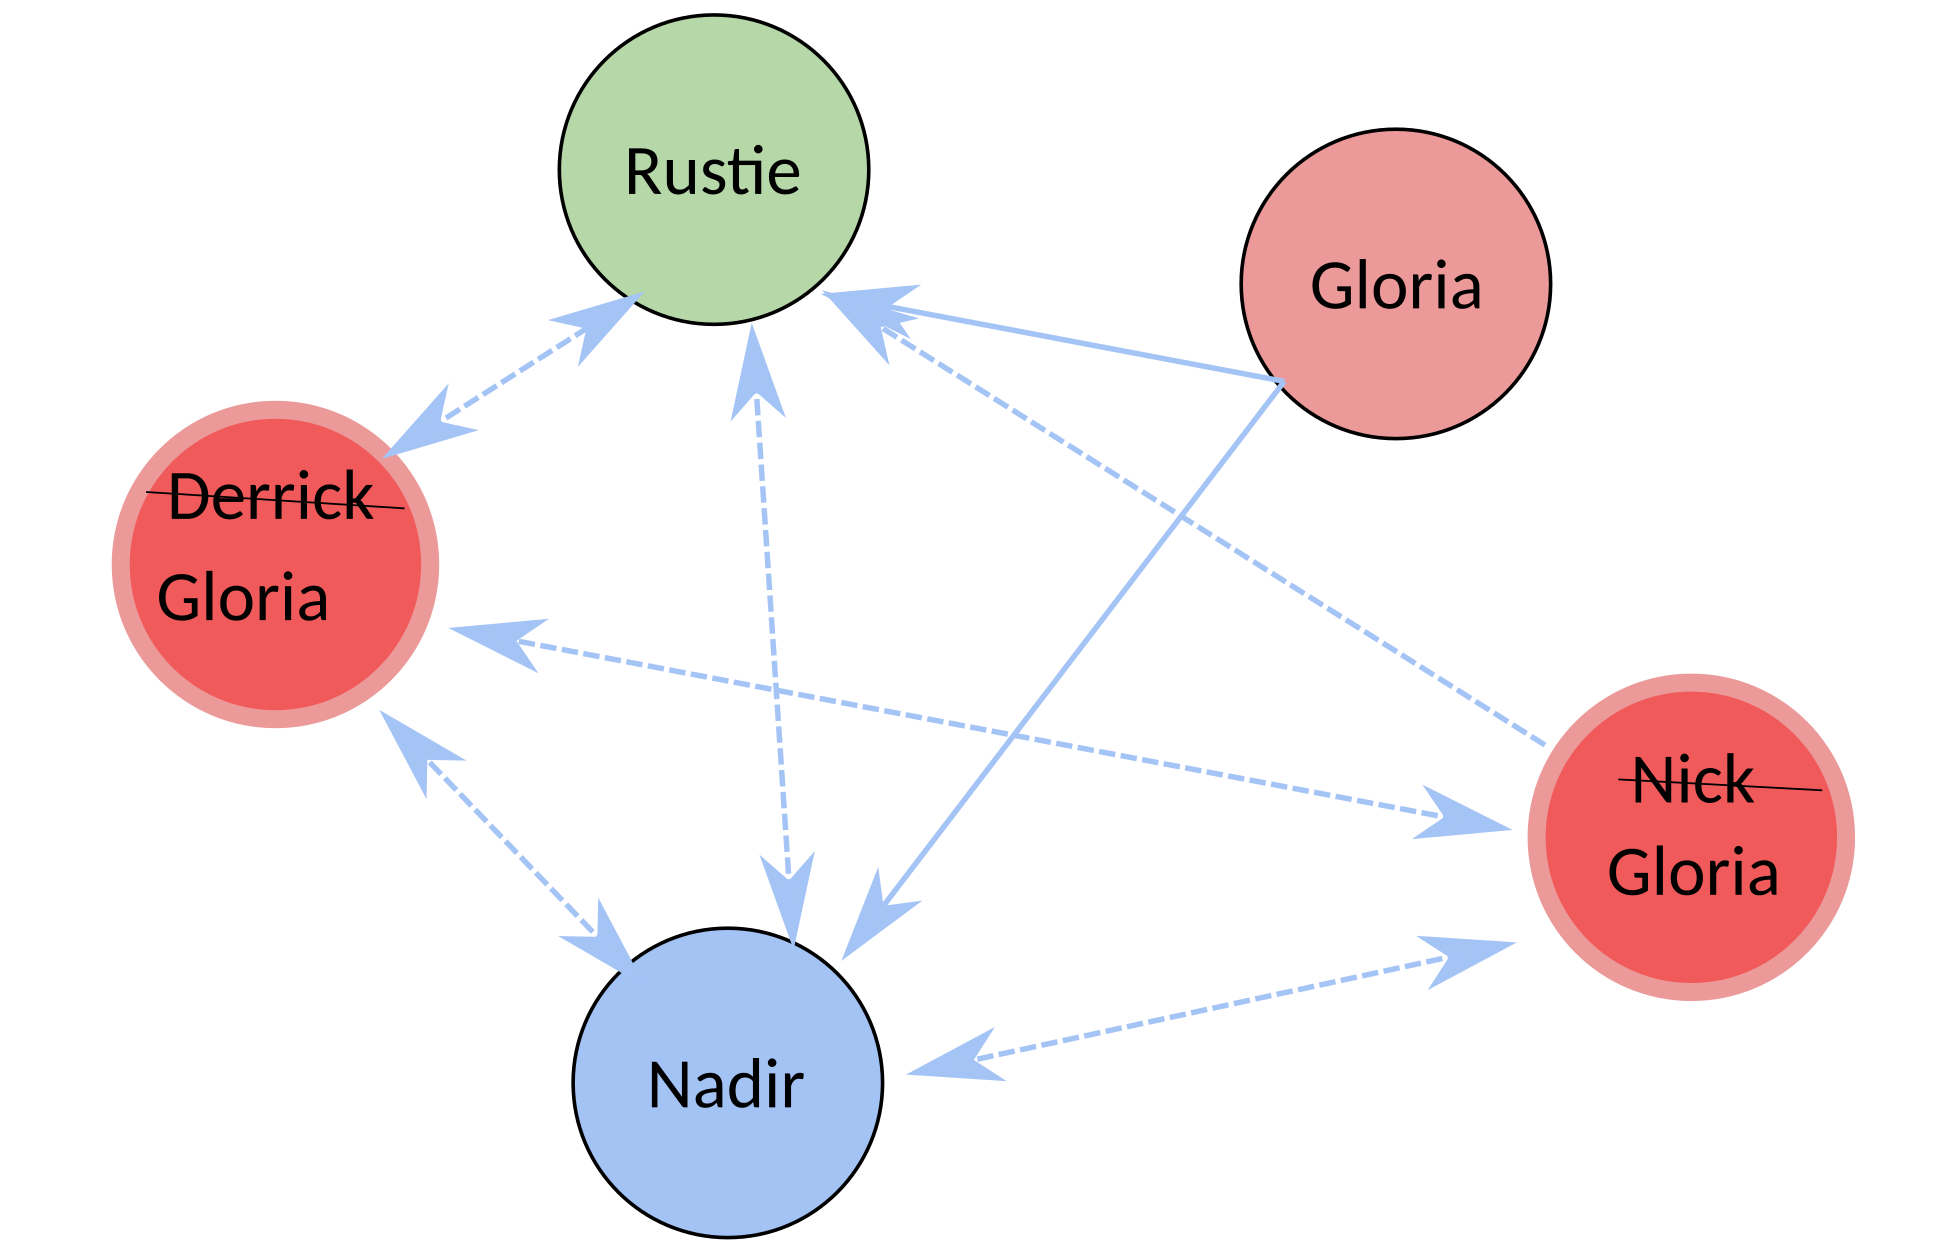
\includegraphics[height=.8\textheight]{Images/consensus6.png}
\end{center}
}
\only<8>{
\begin{center}
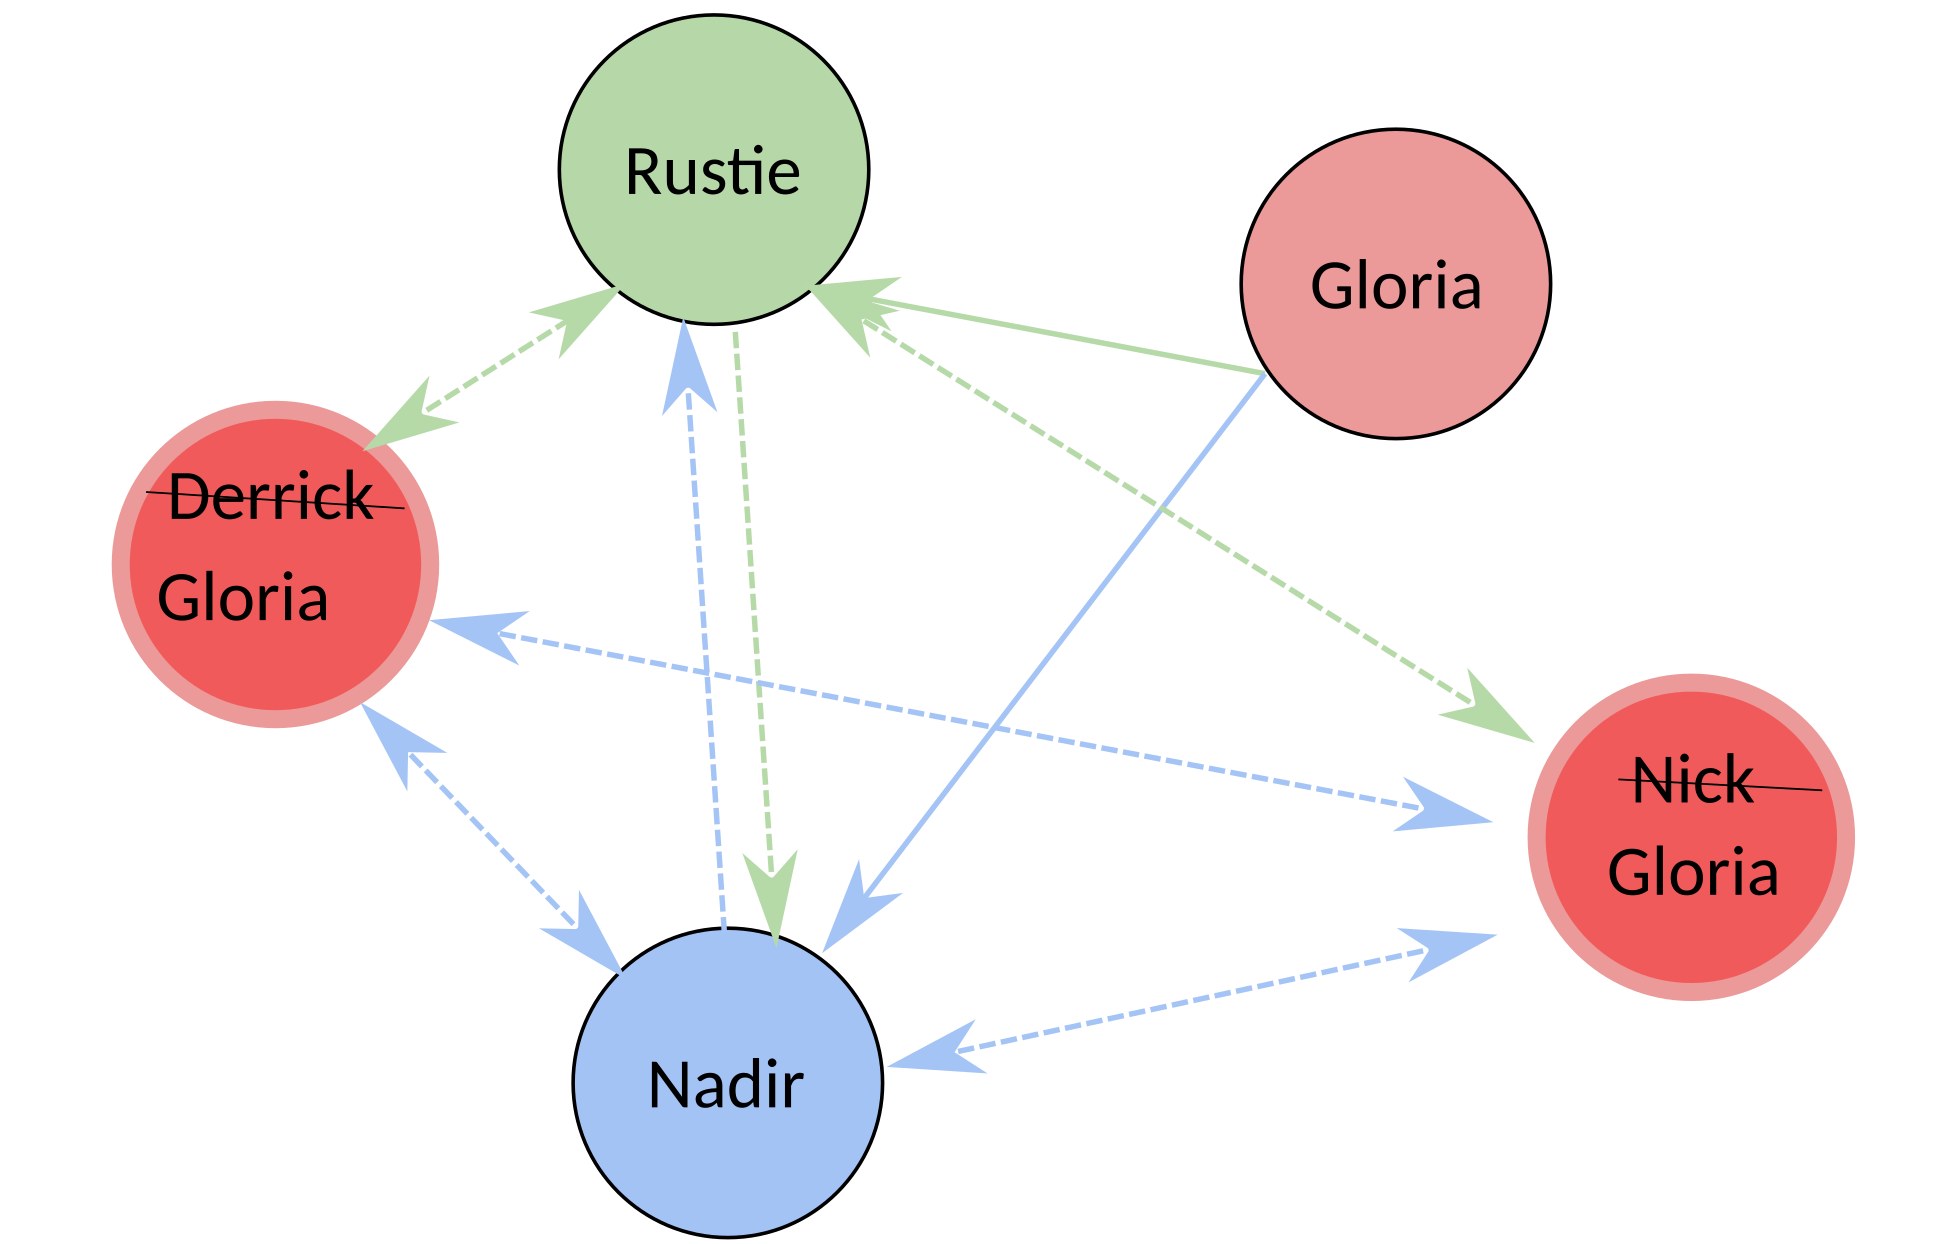
\includegraphics[height=.8\textheight]{Images/consensus7.png}
\end{center}
}
\only<9>{
\begin{center}
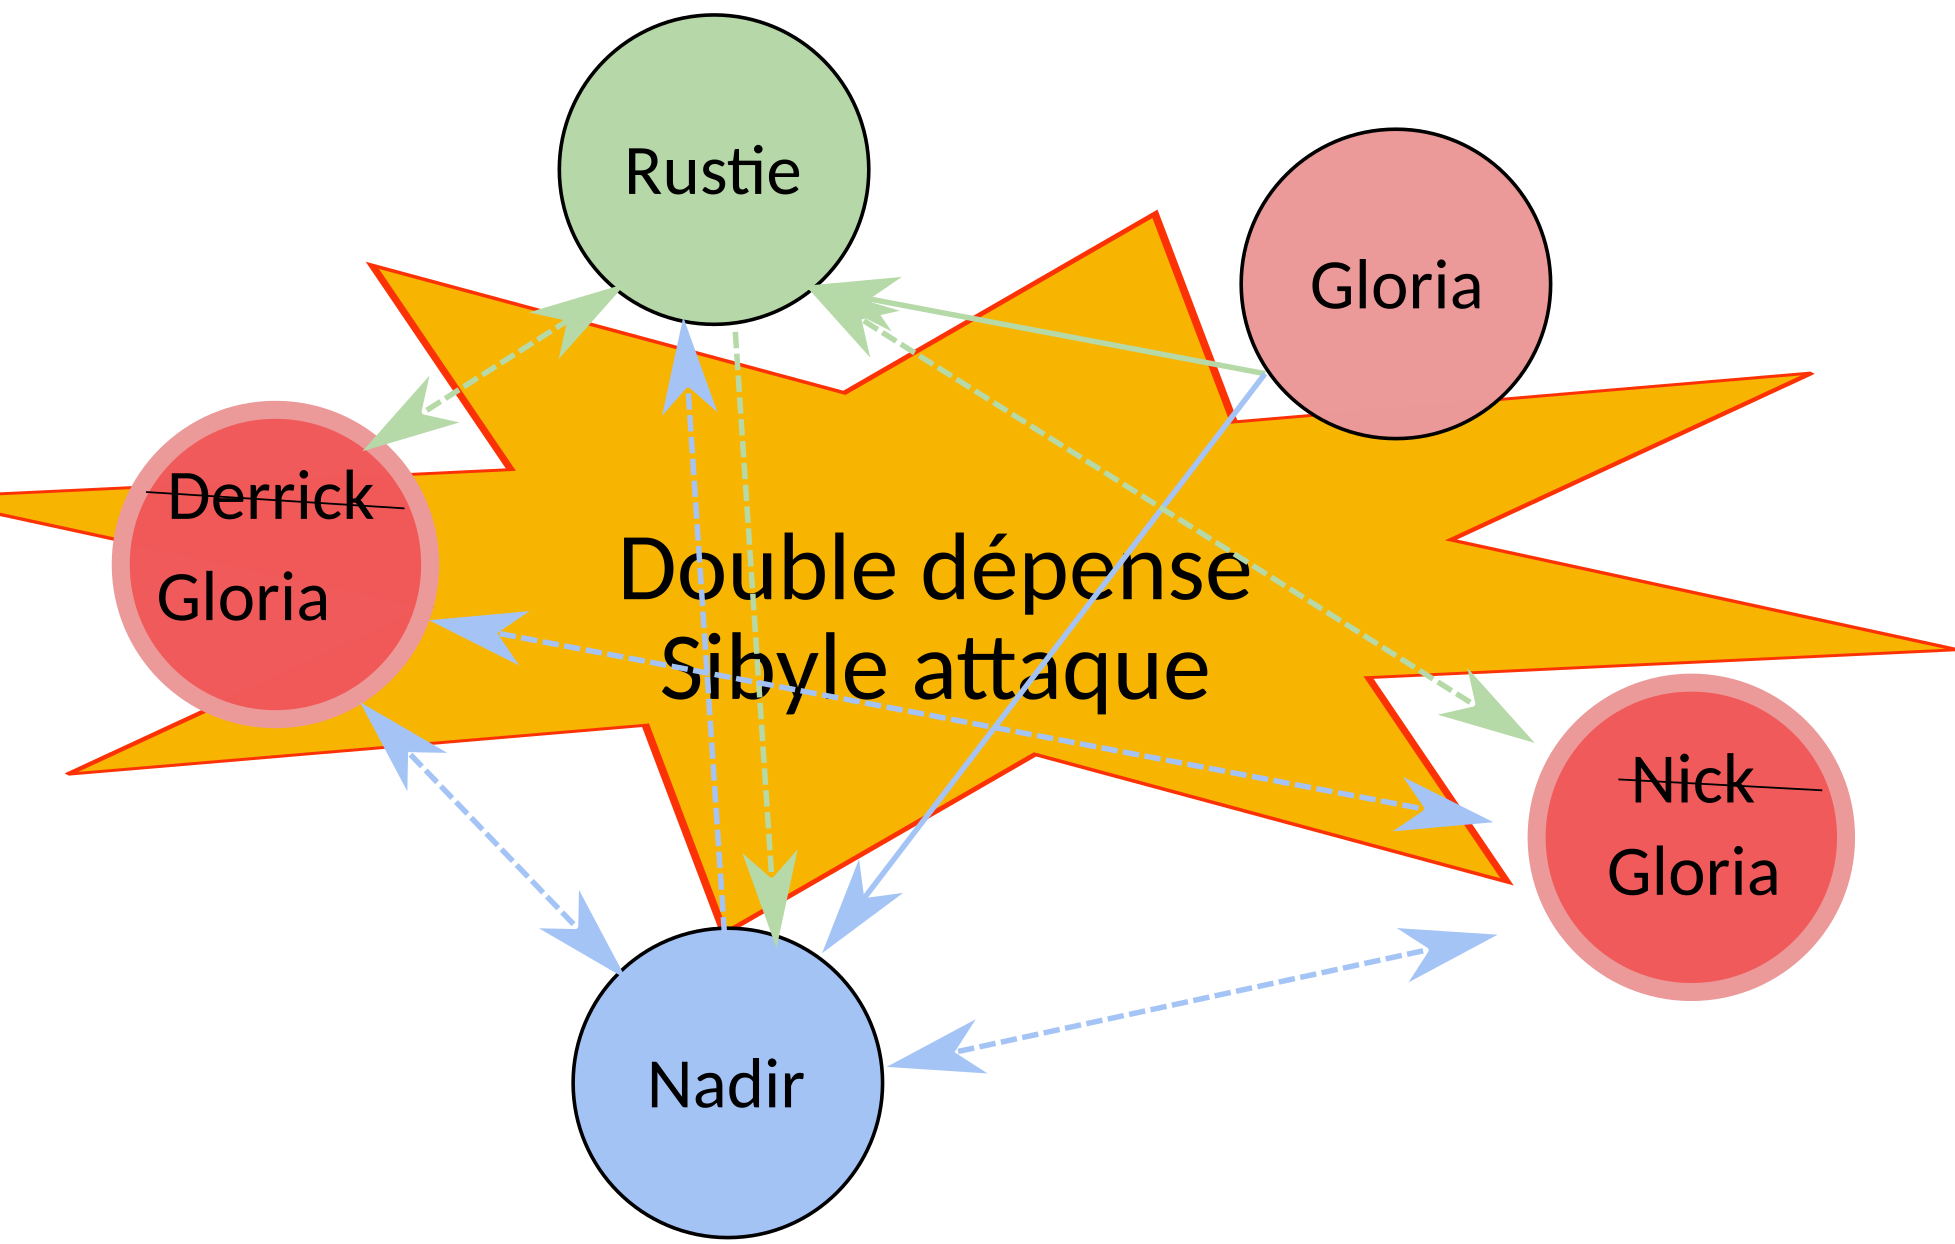
\includegraphics[height=.8\textheight]{Images/consensus8.png}
\end{center}
}
\only<10>{
\begin{center}
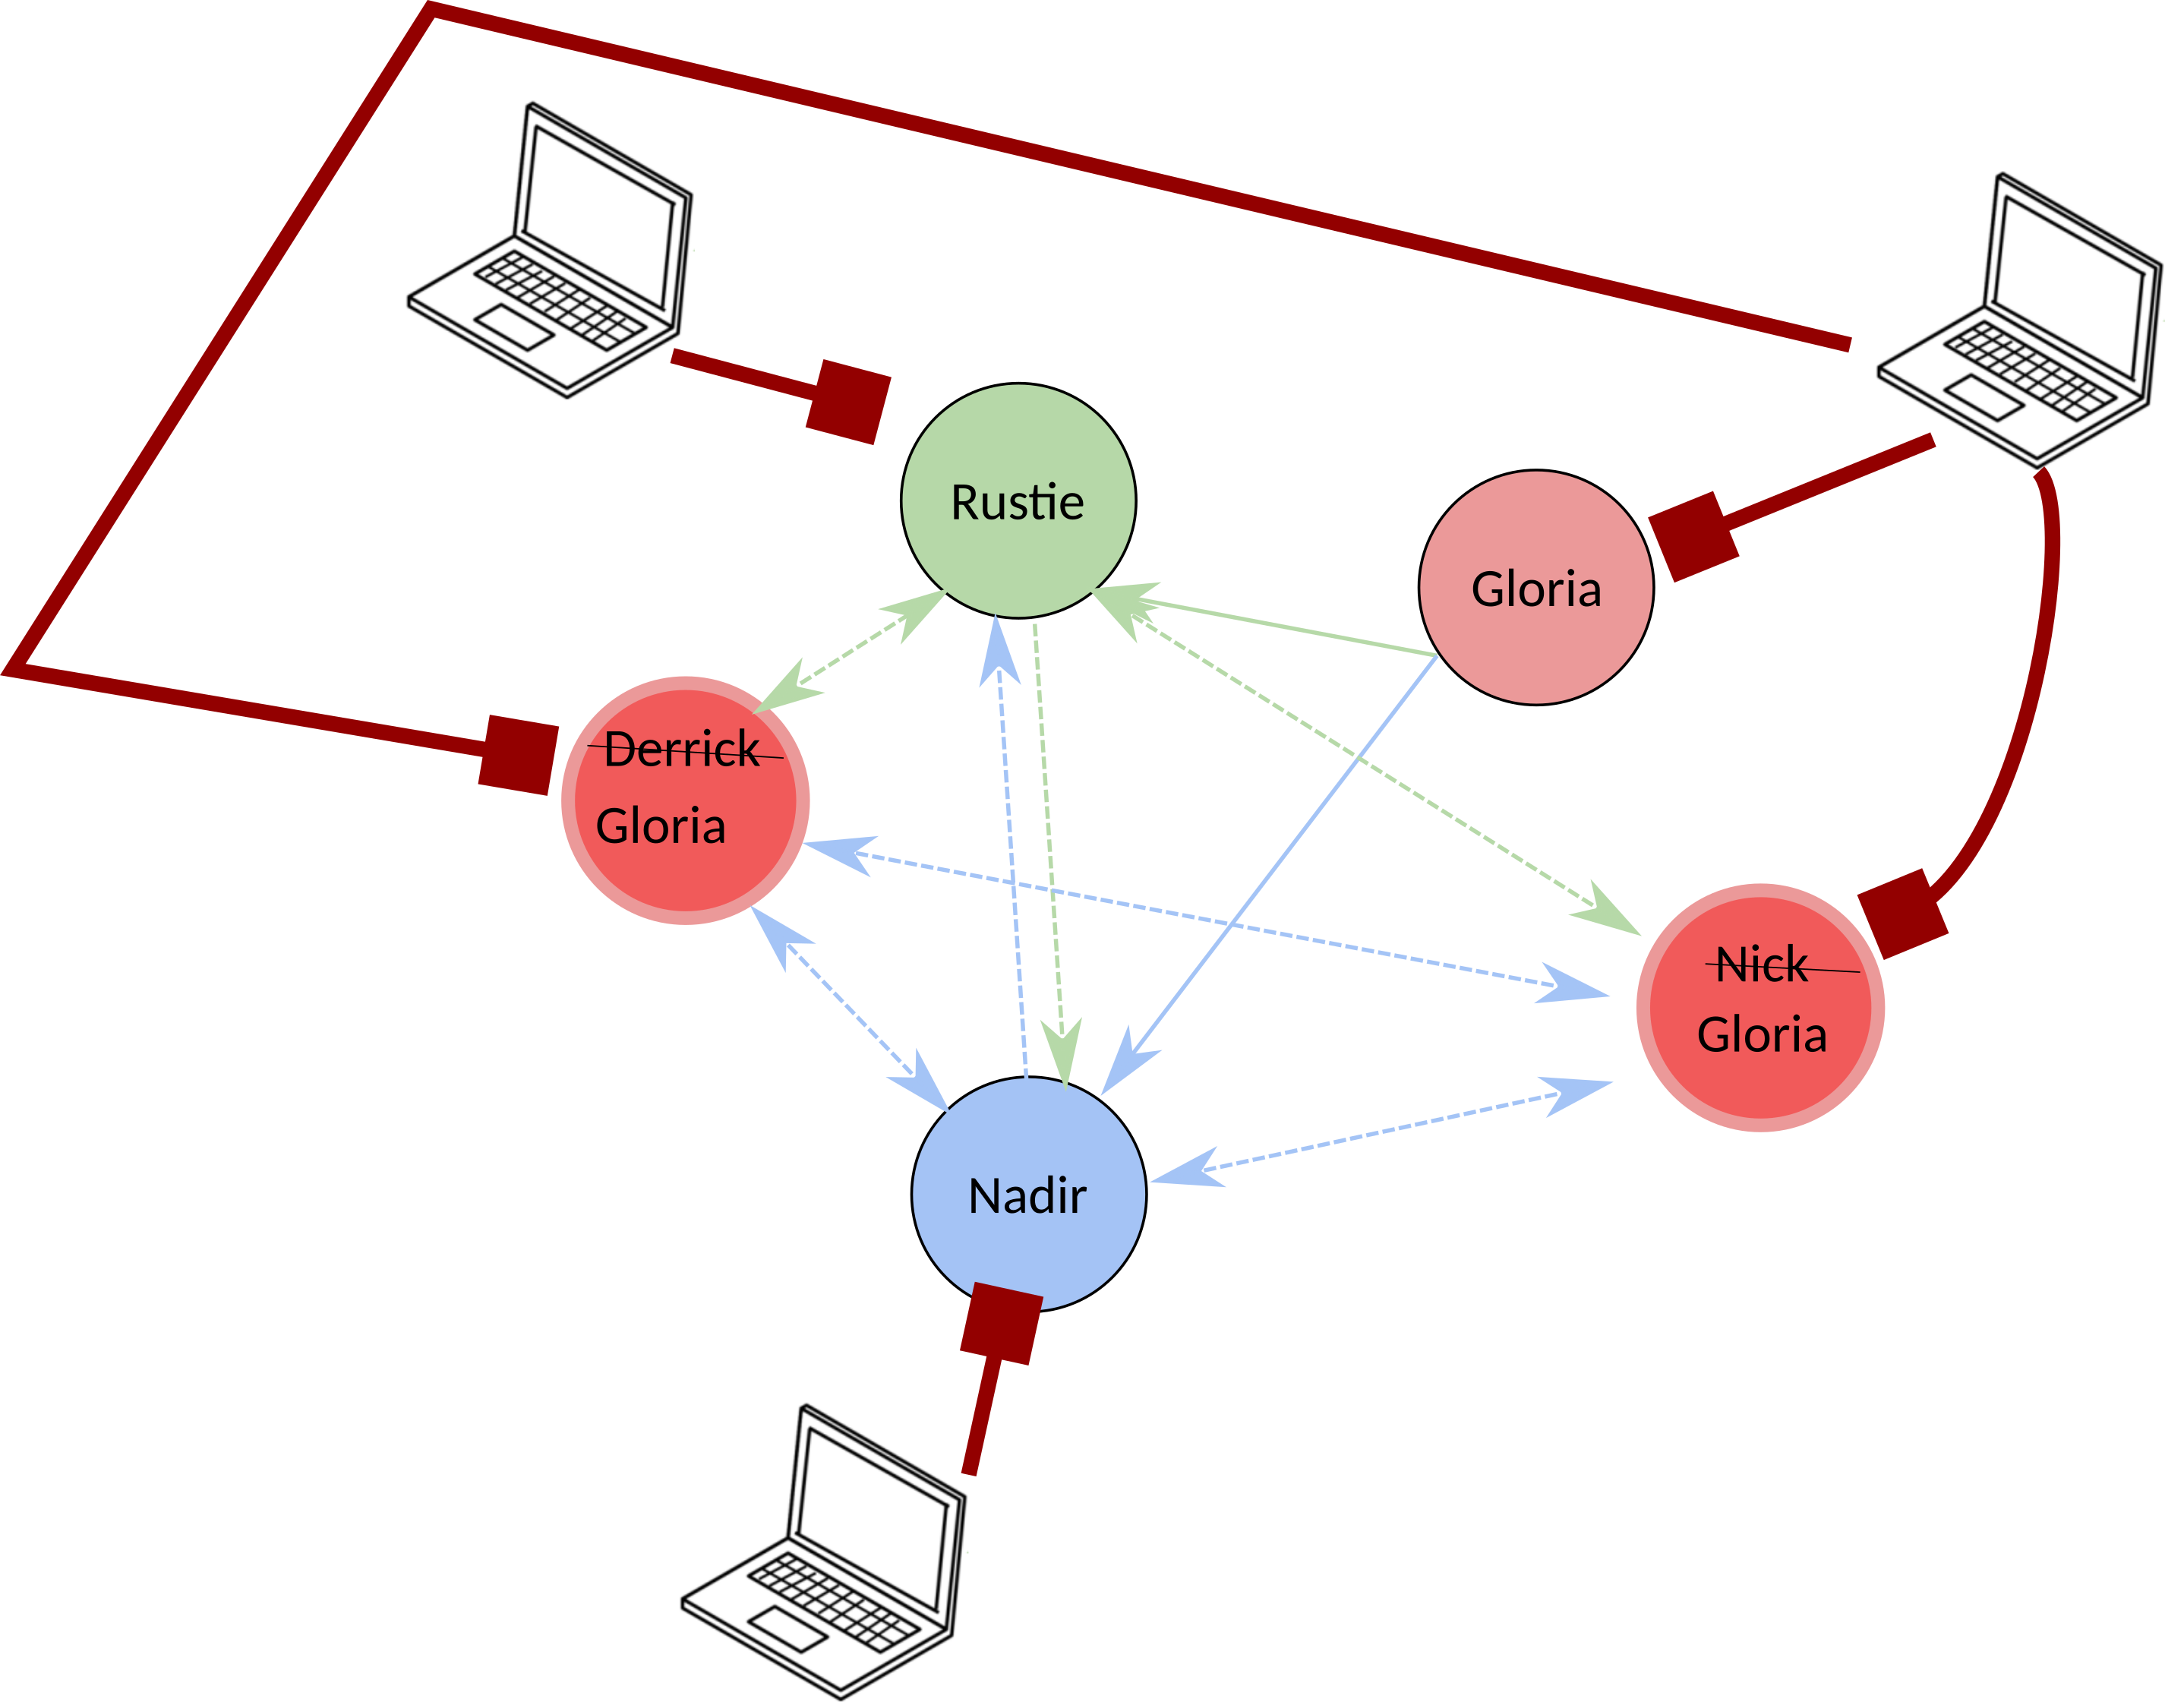
\includegraphics[height=.8\textheight]{Images/consensus9.png}
\end{center}
}

\only<11>{
\begin{center}
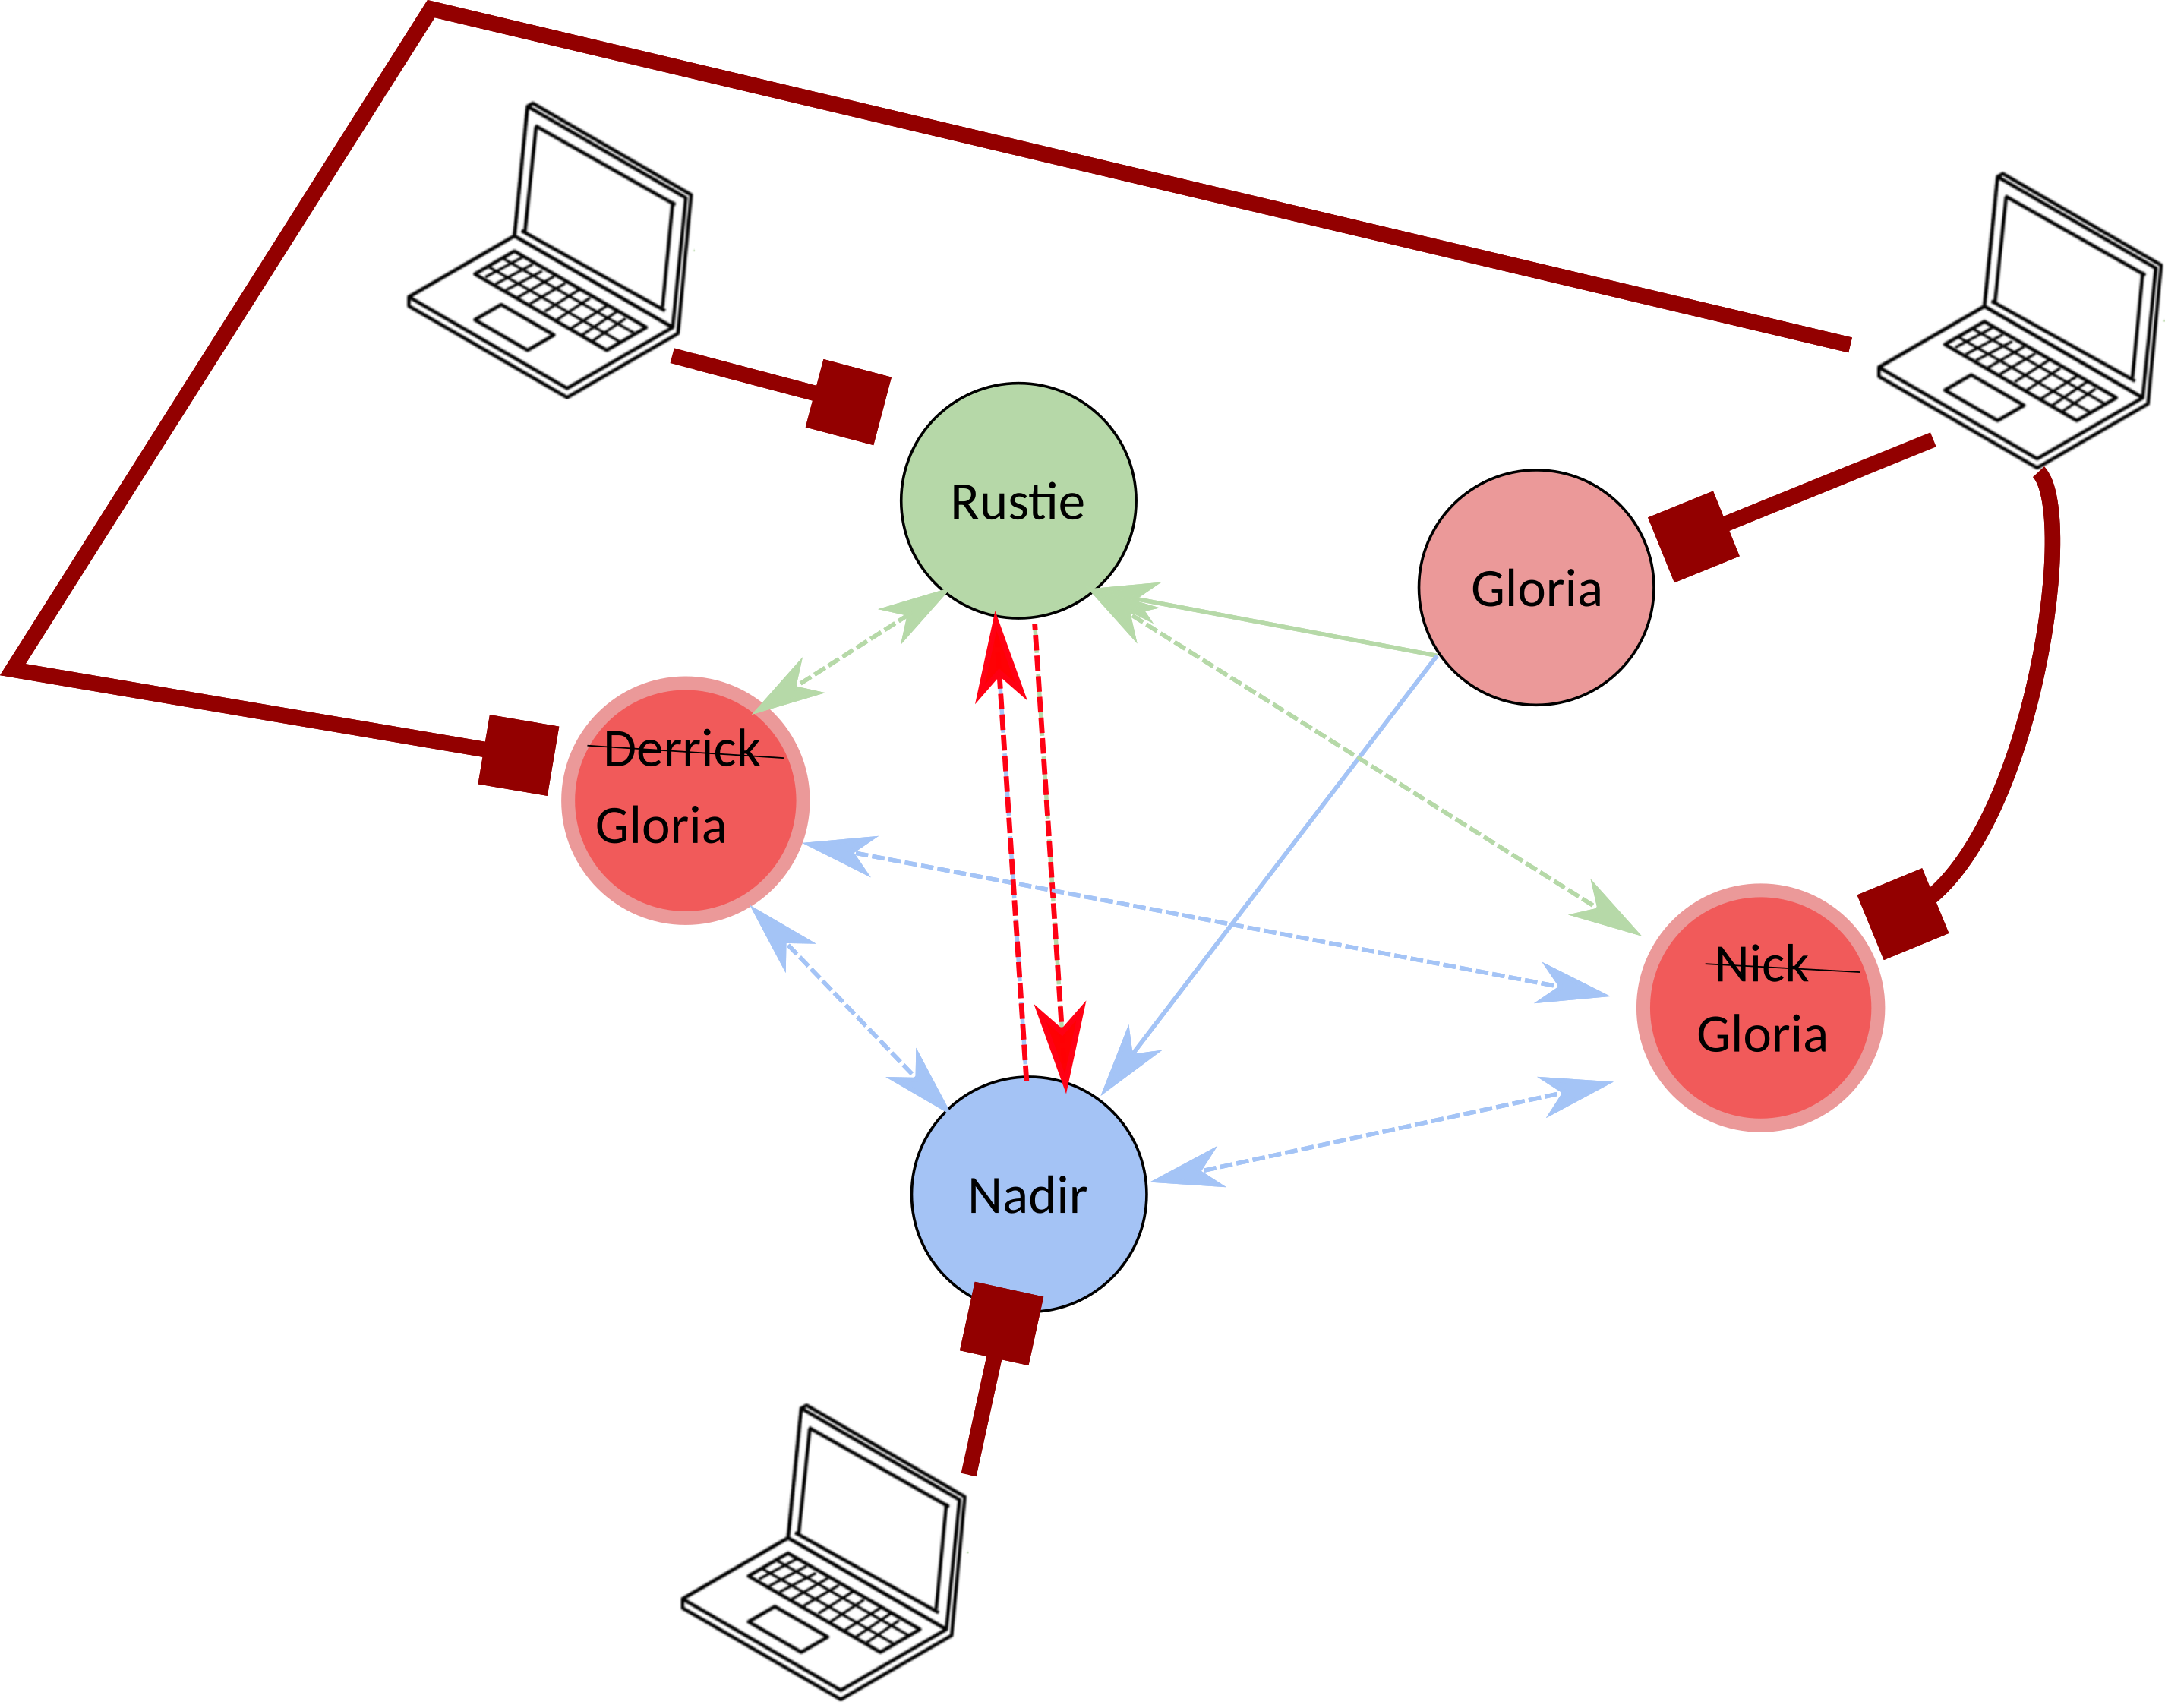
\includegraphics[height=.8\textheight]{Images/consensus10.png}
\end{center}
}


\begin{columns}
\begin{column}{0.50\columnwidth}
\begin{block}<1->{Consensus de Nakamoto}
\begin{itemize}
\item Anonyme et ouvert à tous
\item Règle de la plus longue chaine
\item Leader choisi à la loterie
\item Honnêtes encouragés
\end{itemize}
\end{block}
\end{column}
\begin{column}{0.50\columnwidth}
\begin{block}<1->{}
\end{block}
\end{column}
\end{columns}
\end{frame}

\subsection{Comment maintenir le Consensus autrement ?}
\label{sec:org1b8ffcc}
\begin{frame}[label={sec:org72fbc6c}]{Consensus basé un enjeu}
\begin{columns}
\begin{column}{0.4\columnwidth}
\begin{block}<1->{PoS, DPoS}
\only<1->{
\begin{figure}[htbp]
\centering

\includegraphics[width=.4\textwidth]{Images/ouroboros.png}
\caption{Ouroboros Praos (Cardano)}
\end{figure}
}
\end{block}
\end{column}
\begin{column}{0.6\columnwidth}
\begin{block}<1->{BFT-based POS}
\only<2>{
\begin{figure}[htbp]
\centering

\includegraphics[width=.9\textwidth]{Images/logo_tendermint_text.png}
\caption{Tendermint (Cosmos Hub)}
\end{figure}
}
\only<3>{
\begin{figure}[htbp]
\centering

\includegraphics[width=.9\textwidth]{Images/logo_algorand_text.png}
\caption{Algorand}
\end{figure}
}
\only<4->{
\begin{figure}[htbp]
\centering

\includegraphics[width=.9\textwidth]{Images/logo_casper.png}
\caption{Casper FFG (ETH)}
\end{figure}
}
\begin{itemize}
\item <2-> Tendermint (Cosmos)
\item <3-> Algorand (ALG)
\item <4> Casper FFG (ETH)
\end{itemize}
\end{block}
\end{column}
\end{columns}
\end{frame}
\begin{frame}[label={sec:orgbfd5388}]{D'autres consensus}
\begin{columns}
\begin{column}{0.4\columnwidth}
\begin{block}{}
\begin{itemize}
\item <1-> PoH (Histoire) Solana
\item <2-> Preuve d'espace (Chia)
\item <3-> POA (autorité)
\end{itemize}

\begin{itemize}
\item <4-> PoET (elapsed Time)
\end{itemize}
\end{block}
\end{column}

\begin{column}{0.6\columnwidth}
\begin{block}<1->{}
\only<3->{
\begin{center}

\includegraphics[width=.9\textwidth]{Images/logo_chia_solana.png}
\end{center}
}
\end{block}
\end{column}
\end{columns}

\begin{block}<5->{Consensus Exotique}
\begin{columns}
\begin{column}{0.5\columnwidth}
\begin{block}{}
\begin{itemize}
\item PoH (Preuve de non dépense)
\item PoU (Preuve d'usage)
\end{itemize}
\end{block}
\end{column}
\begin{column}{0.5\columnwidth}
\begin{block}{}
\begin{itemize}
\item PoST (temps d'enjeu)
\item PoL (preuve de vie)
\end{itemize}
\end{block}
\end{column}
\end{columns}
\end{block}
\end{frame}
\begin{frame}[label={sec:org8cbcbb1}]{Vulnérabilité des POS}
\begin{center}
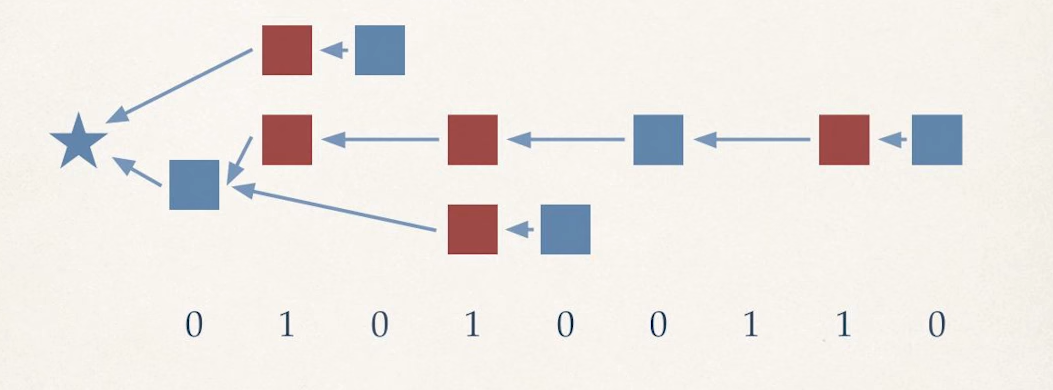
\includegraphics[height=.3\paperheight]{Images/longuest_chain.png}
\end{center}

\begin{block}{Simulation gratuite}
\begin{itemize}
\item Il n'y rien en jeu
\item Corruption postérieur
\item Attaque longue distance (long range attack)
\end{itemize}

\begin{itemize}
\item Trafic sur l'enjeu  (stake grinding attack)
\end{itemize}
\end{block}
\end{frame}



\begin{frame}[label={sec:org6284eb0}]{Optimisations}
\begin{block}{Le trilemme}
\begin{center}
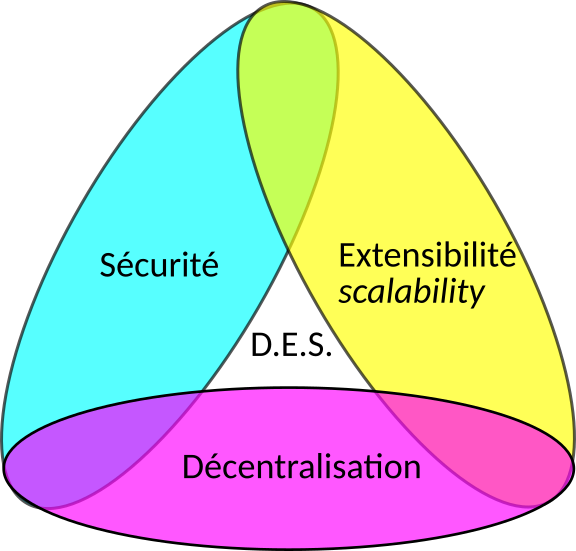
\includegraphics[width=.7\paperheight]{Images/trilemme_ven.png}
\end{center}
\end{block}
\end{frame}

\begin{frame}[label={sec:org0e58eaa}]{Optimisations}
\begin{columns}
\begin{column}{0.46\columnwidth}
\begin{block}<1->{Vitesses : Segwit}
\only<1>{
\begin{center}
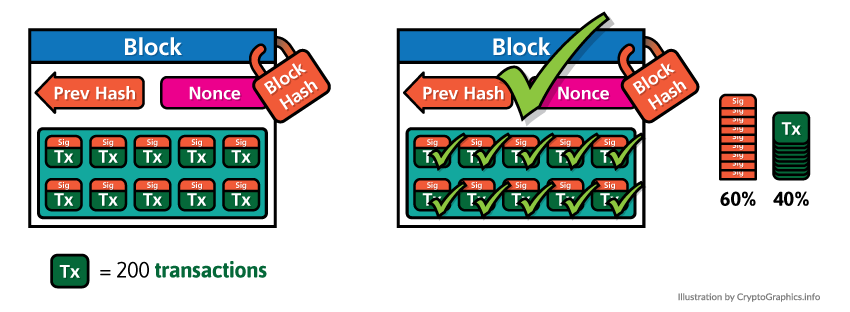
\includegraphics[width=\textwidth]{Images/segWit-1.png}
\end{center}
}
\end{block}
\end{column}
\begin{column}{0.46\columnwidth}
\begin{block}<1->{Vitesses : Segwit 2x}
\begin{center}
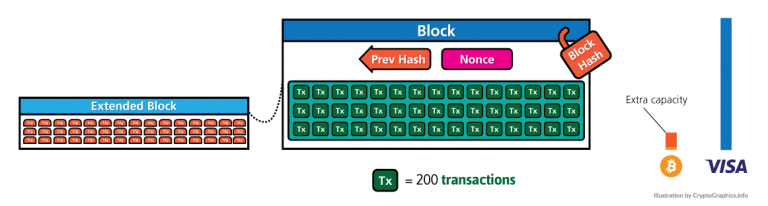
\includegraphics[width=\textwidth]{Images/segWit2x.png}
\end{center}
\end{block}
\end{column}
\end{columns}

\begin{block}{Vitesses : Améliorations lightning}
\begin{center}
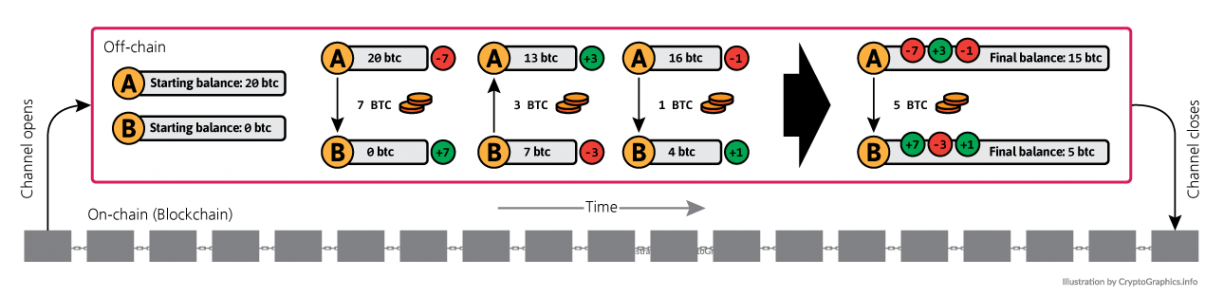
\includegraphics[width=\textwidth]{Images/payment-channels.png}
\end{center}
\end{block}
\end{frame}




\section{Perspectives}
\label{sec:orgec75651}
\subsection{Perspectives}
\label{sec:org4dd5a07}
\begin{frame}[label={sec:org6c58303}]{}
\begin{itemize}
\item Comment maintenir les consensus ?
\item Cryptographie à l'épreuve des ordinateurs quantiques ?
\item Quelle avenir pour les blockchains publiques ?
\end{itemize}
\end{frame}
\begin{frame}[label={sec:org3d009df}]{}
\begin{block}{Merci}
{
  \usebackgroundtemplate{\includegraphics[height=\paperheight]{./remerciement}}
  \frame[plain]{
  }
}
\end{block}
\end{frame}
\end{document}